\section{Le second principe}

	\subsection{Énoncé}
	\label{ch_second_principe_enonce}

		Le \vocab{second principe de la thermodynamique} s’exprime ainsi :

		\begin{principe}
			La chaleur ne se déplace spontanément que vers une température plus basse.
		\end{principe}

		On peut préciser cette affirmation de la façon suivante :

		\begin{trucimportant}
			Le transfert de chaleur vers une température plus haute\linebreak
			ne peut se faire sans apport d’énergie.
		\end{trucimportant}

		Nous allons voir que ce simple constat a des conséquences multiples et profondes pour l’ingénieur/e. En particulier, il détermine l’efficacité maximale de tous les moteurs et réfrigérateurs !



	\subsection{De l’évidence du second principe}

		L’énoncé ci-dessus paraît si évident qu’on peut presque s’en offusquer. Deux remarques s’imposent ici.

		\begin{itemize}
			\item Le second principe peut être énoncé de multiples façons. Il est plus impressionnant de parler d’«~accroissement de l’entropie~» que du comportement spontané de la chaleur ; pourtant ces différents énoncés, que nous allons aborder progressivement, sont tous équivalents.
			\item L’apparente évidence manifeste du postulat --\ on se doute que nul n’a jamais vu de tasse de thé chaud se réchauffer spontanément, ni de boisson fraîche se refroidir seule à température ambiante\ -- s’effrite dès que l’on étudie les phénomènes à l’échelle microscopique. 

		En effet, si la température n’est que le niveau d’agitation des particules, alors rien n’empêche \textit{a priori} celle-ci d’augmenter localement même si la température ambiante est plus faible\footnote{L’étudiant/e curieux/se pourra explorer cette idée en étudiant l’expérience intrigante du \textit{\wfd{Démon de Maxwell}{démon de Maxwell}}, qui ouvre les portes vers de nombreux nouveaux concepts.}. Il a fallu un demi-siècle de travail ardu aux thermodynamiciens pour répondre à cela de façon satisfaisante\footnote{C’est l’application des probabilités et statistiques à la thermodynamique, et en particulier le travail de Ludwig Boltzmann (\S\ref{ch_entropie_boltzmann}), qui permettra de la réconcilier avec la vision mécanistique Newtonienne du monde, au cours du \textsc{xx}\ieme siècle.}. Il ne s’agit pas d’un problème trivial.
		\end{itemize}

		Dans notre étude et depuis notre point de vue d’ingénieur/e, nous accepterons le postulat ci-dessus comme une évidence, sans chercher ni à le justifier, ni à l’expliquer.
		
		
	\subsection{Principe zéro et troisième principe}
	
		Le \wed{Zeroth law of thermodynamics}{\vocab{principe zéro}} de la thermodynamique stipule que si deux corps sont en équilibre thermique avec un troisième, alors tous les trois sont en équilibre l’un avec l’autre. Le \wfd{Troisième principe de la thermodynamique}{\vocab{troisième principe}} stipule que l’entropie (une propriété que nous étudions au chapitre prochain) d’un cristal à température zéro est nulle. Ni l’un ni l’autre ne revêt la moindre importance pour l’ingénieur/e.



\section{Le second principe et les machines thermiques}
\label{ch_second_principe_machines_thermiques}

	\subsection{Tous les moteurs rejettent de la chaleur}
	\label{ch_demo_second_principe}

		Imaginons qu’on veuille créer du travail en prenant de la chaleur à un objet «~chaud~», c’est-à-dire à haute température : par exemple, \SI{100}{\degreeCelsius}, comme montré en \cref{fig_démo_second_principe_1}. On accole à cet objet un cylindre empli d’un fluide, et on laisse le fluide pousser sur un piston au fur et à mesure qu’il reçoit de la chaleur.

		\begin{figure}
			\begin{center}
				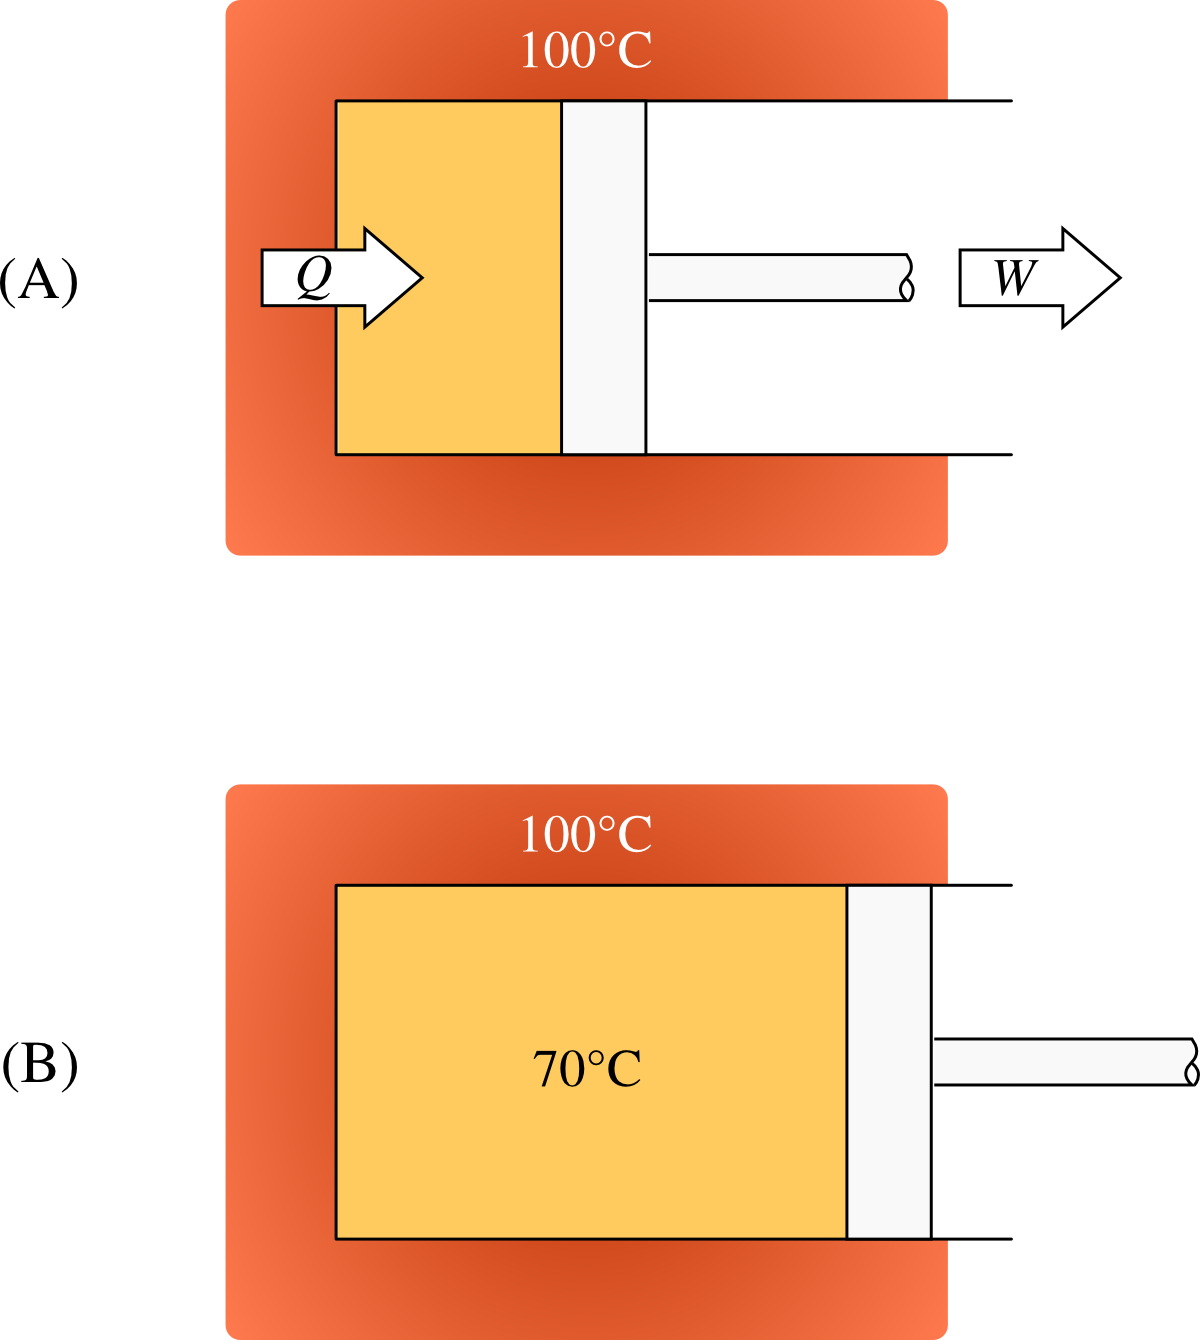
\includegraphics[width=8cm]{images/demo_second_principe_1.png}
			\end{center}
			\supercaption{Production d’un travail avec de la chaleur issue d’un corps à~\SI{100}{\degreeCelsius} : le transfert de chaleur permet la production d’un travail mais il provoque également une augmentation de température du fluide.}{schéma \cczero \oc}
			\label{fig_démo_second_principe_1}
		\end{figure}

		Une fois qu’une quantité de travail a été fournie (en B sur la \cref{fig_démo_second_principe_1}), le fluide a augmenté de volume. Si nous souhaitons continuer à transformer de la chaleur en travail et que nous ne souhaitons pas que le moteur «~gonfle~» indéfiniment, il nous faut refroidir ce gaz pour le ramener à son volume initial.

		\thermoquotebegin{O}
			D’après ce principe, il ne suffit pas, pour donner naissance à la puissance motrice, de produire de la chaleur : il faut encore se procurer du froid ; sans lui la chaleur serait inutile.\\
			Et en effet, si l’on ne rencontrait autour de soi que des corps aussi chauds que nos foyers, comment parviendrait-on à condenser la vapeur ? Où la placerait-on une fois qu’elle aurait pris naissance ? Il ne faudrait pas croire que l’on pût, ainsi que cela se pratique dans certaines machines, la rejeter dans l’atmosphère : l’atmosphère ne la recevrait pas. Il ne la reçoit, dans l’état actuel des choses, que parce qu’il remplit pour elle l’office d’un vaste condenseur, parce qu’il se trouve à une température plus froide : autrement il en serait bientôt rempli, ou plutôt il en serait d’avance saturé.%
		\thermoquoteend{Sadi Carnot, 1824~\cite{carnot1824}}{\onlyframabook{\vspace{3em}}}%handmade

		Malheureusement, \emph{la seule façon} d’extraire de la chaleur du gaz est de le mettre en contact avec un corps plus «~froid~», comme montré en \cref{fig_démo_second_principe_2}. En particulier, il est impossible de restituer la chaleur accumulée dans le gaz au corps «~chaud~» --\ il faudrait pour cela que la température du gaz soit plus grande que lui\footnote{Notons qu’en poussant le raisonnement à ses limites, le moteur pourrait recevoir et fournir la chaleur à température constante. Mais alors, le travail à fournir pour ramener le fluide à son état initial serait exactement le même que celui développé pendant la détente : le cycle ne transformerait effectivement pas de chaleur en travail, et ne présenterait alors pas d’intérêt pratique.}. Cette chaleur accumulée est donc irrémédiablement perdue.

		\begin{figure}
			\begin{center}
				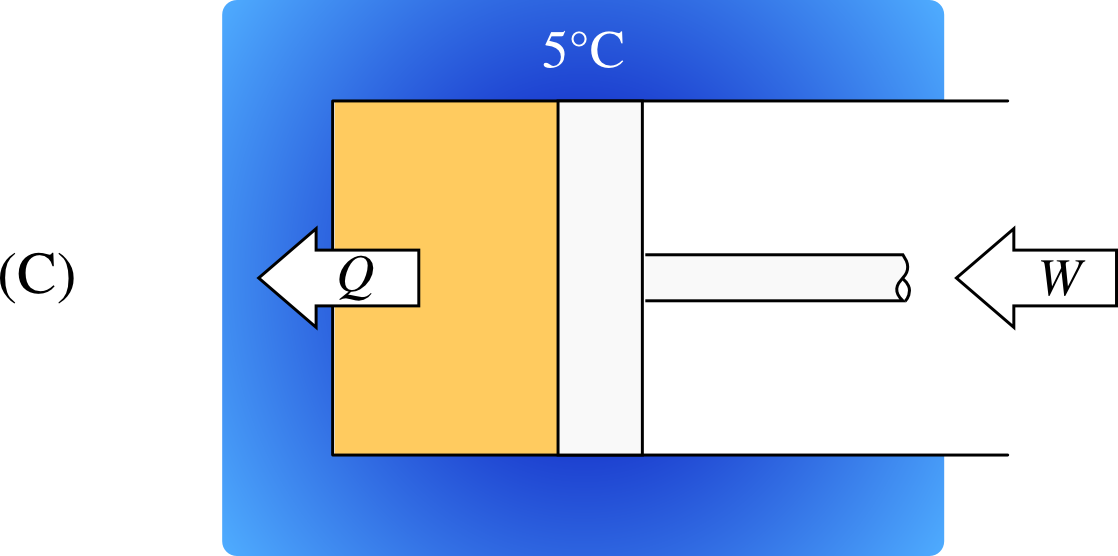
\includegraphics[width=7.2cm]{images/demo_second_principe_2.png}
			\end{center}
			\supercaption{Le refroidissement inévitable du moteur.
		La seule manière de ramener le fluide à son état initial (A) dans l’expérience en \cref{fig_démo_second_principe_1} est de lui prélever de la chaleur, ce qui ne peut se faire qu’avec un «~puits~» à chaleur de température plus basse. Les transferts de chaleur et de travail sont ici plus faibles qu’à l’aller, mais tous deux non nuls.}{schéma \cczero \oc}
			\label{fig_démo_second_principe_2}
		\end{figure}

		Ainsi, pour qu’un moteur fonctionne en continu, il faut qu’en plus d’une source à haute température où capter de la chaleur, il dispose d’un «~puits~» à faible température, où rejeter la chaleur dont il ne peut plus rien faire.

		Ce raisonnement s’applique de la même façon aux machines conçues pour absorber de la chaleur à basse température (réfrigérateurs, climatiseurs, et pompes à chaleur). Une fois que la chaleur a été captée dans le fluide à basse température, la seule façon de la rejeter à une température plus haute est d’augmenter la température du fluide. Cela nécessite un travail de compression non-nul. Ainsi, pour qu’un réfrigérateur fonctionne en continu, il faut qu’il reçoive de l’énergie sous forme de travail.


	\subsection{Limites des machines thermiques}
	\label{ch_limites_machines_thermiques}
	
		Pour étudier plus rigoureusement les transformations de chaleur et de travail, nous utiliserons la notation suivante pour décrire les machines thermiques :

		\begin{itemize}
			\item $T_H$ et $T_B$ représenteront respectivement les températures haute et basse ;
			\item Nous appellerons toujours $\dot Q_{TH}$ la puissance sous forme de chaleur transmise à haute température, et $\dot Q_{TB}$ son équivalente à basse température (elles peuvent chacune être de signe positif ou négatif).
		\end{itemize}

		Ainsi la machine thermique dans sa représentation la plus générale ressemble à la \cref{fig_conventions_notation_machines_thermiques}.

		Il est très important de souligner que quels que soient le mode de fonctionnement et l'efficacité de la machine, elle ne peut ni créer ni détruire de l’énergie (\S\ref{ch_premier_principe}) ; et nous aurons toujours :
		\begin{equation}
			\dot Q_{TH} + \dot Q_{TB} + \dot W_\net = 0
			\label{eq_premier_principe_machines}
		\end{equation}

		\begin{figure}%[h] % positionning sucks otherwise, for some reason
			\begin{center}
				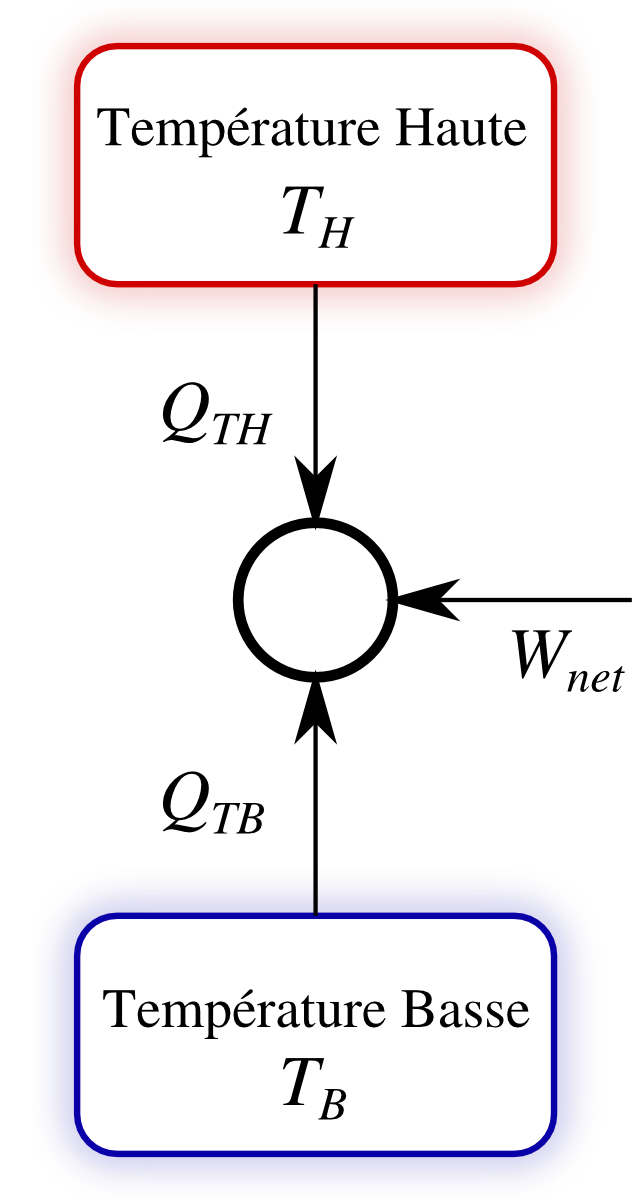
\includegraphics[height=8cm]{images/moteur_forme_generale.png}
			\end{center}
			\supercaption{Une machine thermique transformant travail et chaleur dans sa représentation la plus générale.}{schéma \cczero \oc}
			\label{fig_conventions_notation_machines_thermiques}
		\end{figure}

		\clearfloats
		Le second principe a des conséquences particulières pour chacun des deux grands types de machines thermiques :

		\begin{description}

			\item[Un moteur]{prélève de la chaleur à une source à haute température ($\dot Q_{TH} > 0$) et produit un travail ($\dot W_\net < 0$, \cref{fig_moteur_exemple_valeurs}). Nous venons de voir que si nous voulons effectuer cette transformation en continu, nous n’avons d’autre choix que de rejeter de la chaleur dans un réservoir à basse température ($\dot Q_{TB} < 0$).

			\begin{figure}
				\begin{center}
					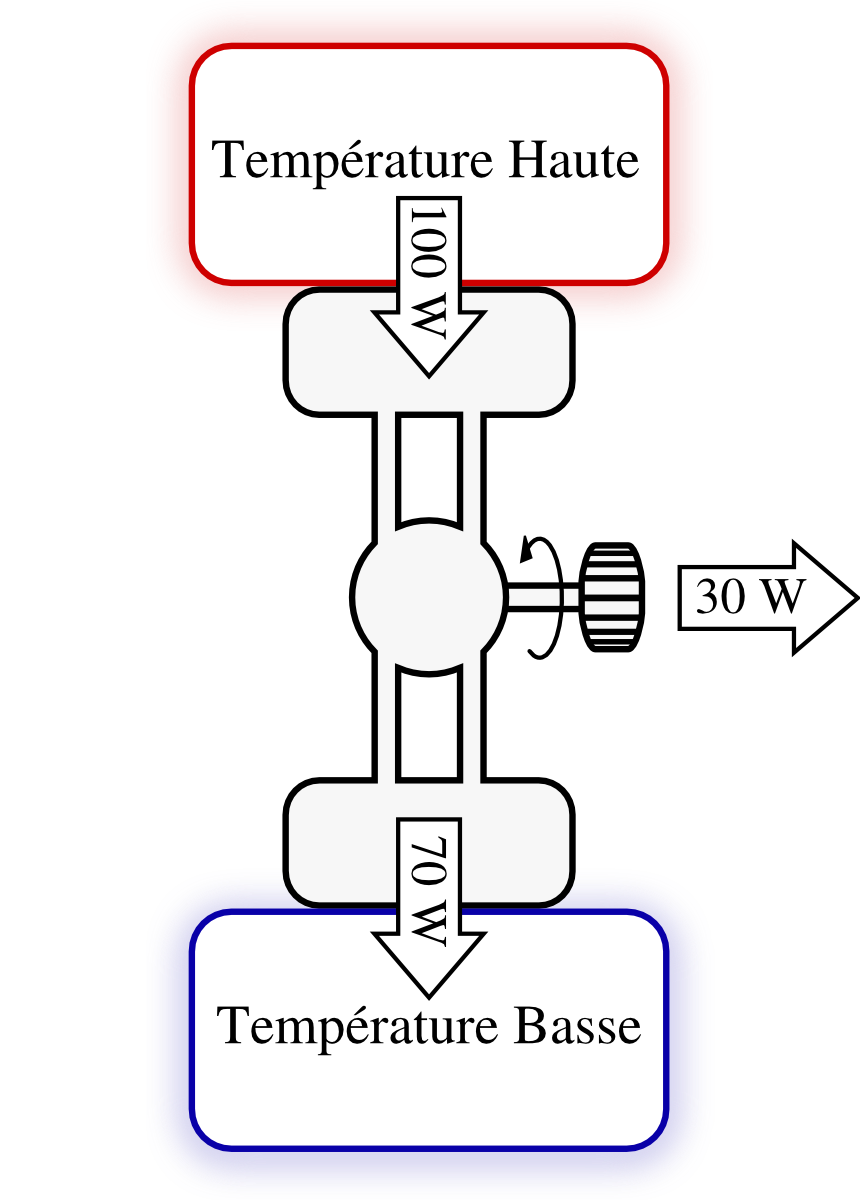
\includegraphics[height=8cm]{images/exemple_moteur.png}
				\end{center}
				\supercaption{Un exemple de transferts énergétiques vers un moteur thermique. }{schéma \cczero \oc}
				\label{fig_moteur_exemple_valeurs}
			\end{figure}

			Dans les centrales électriques, les deux zones de température sont identifiables facilement : la vapeur prélève de la chaleur au cœur de la centrale (réacteur nucléaire, chaudière à gaz ou à charbon) et rejette de la chaleur par les larges cheminées de refroidissement.

			Les moteurs automobiles et aéronautiques, quant à eux, doivent vidanger l’air qui leur sert de fluide de travail à cause des produits de combustion qui empêchent leur ré-utilisation. Pour cette raison, le refroidissement a lieu dans l’atmosphère, en dehors de la carcasse du moteur. Leur «~zone de refroidissement~» n’est pas distinguable facilement.

			Appliqué au moteur, le second principe peut s’exprimer ainsi :

			\begin{trucimportant}
			Aucun moteur ne peut transformer continûment\linebreak
			de la chaleur en travail\linebreak
			à partir d’une seule source de chaleur.\linebreak
			Tous les moteurs rejettent de la chaleur à plus faible température.\linebreak
			\end{trucimportant}
			\begin{trucimportant}
			Le fonctionnement en continu d’un moteur\linebreak
			nécessite deux réservoirs de chaleur, chacun de température différente.
			\end{trucimportant}

			Les puristes exprimeront ce corollaire, dit \vocab{de Kelvin-Planck}, avec l’inéquation suivante :
			\begin{equation}
				\dot Q_{TH} > -\dot W_\net
			\end{equation}
			\begin{equationterms}
				\item pour tout moteur thermique.
			\end{equationterms}

		}%end item

		\clearfloats
		\item[Un réfrigérateur, un climatiseur ou une pompe à chaleur]{a un fonctionnement inverse à celui des moteurs. Ces machines extraient de la chaleur d’une source à basse température ($\dot Q_{TB} > 0$) pour la rejeter dans un réservoir à plus haute température ($\dot Q_{TH} < 0$, \cref{fig_refrigerateur_exemplevaleurs}). Une conséquence inévitable est qu’elles consomment pour cela du travail ($\dot W_\net > 0$).

			\begin{figure}
				\begin{center}
					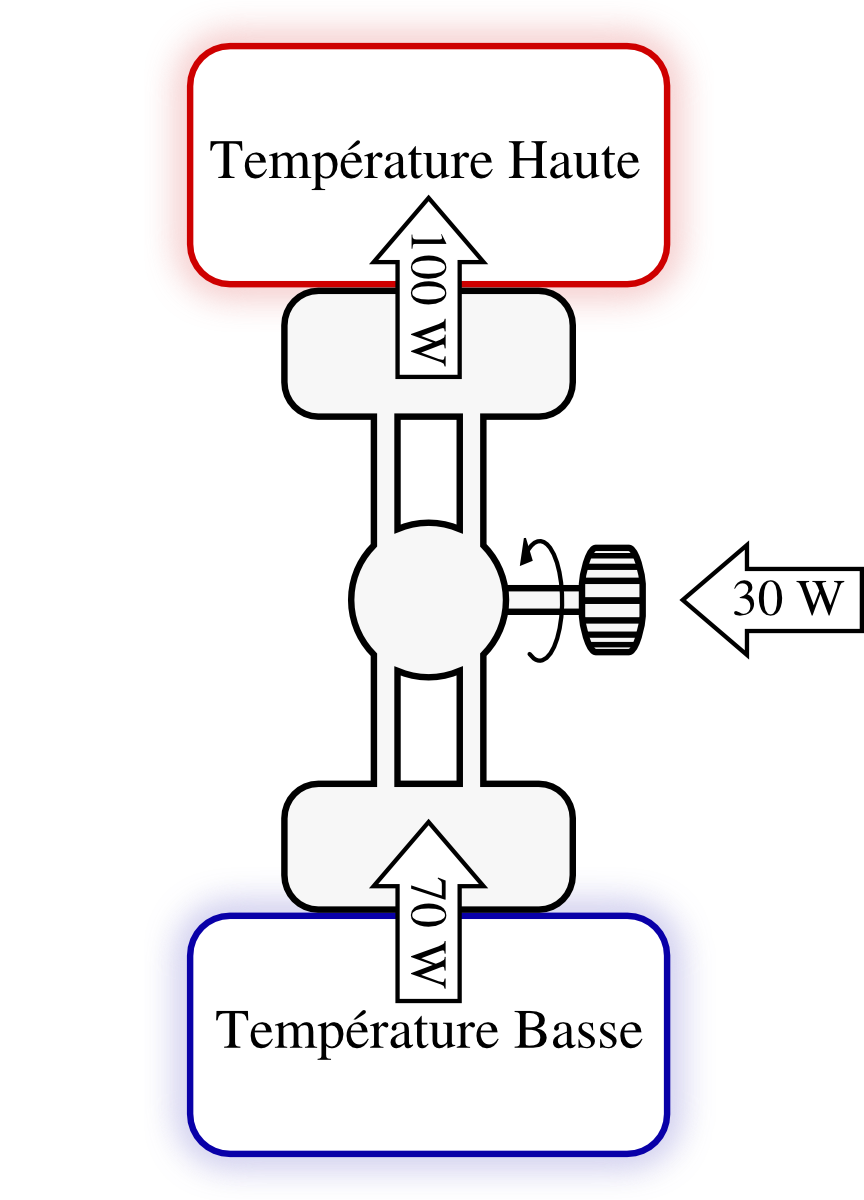
\includegraphics[height=8cm]{images/exemple_refrigerateur.png}
				\end{center}
				\supercaption{Un exemple de transferts énergétiques en jeu dans un réfrigérateur, un climatiseur ou une pompe à chaleur en fonctionnement.}{schéma \cczero \oc}
				\label{fig_refrigerateur_exemplevaleurs}
			\end{figure}

			Appliqué à un réfrigérateur, le second principe s’exprime ainsi :

			\begin{trucimportant}
			Toute machine transférant de la chaleur depuis un corps vers un autre de température plus haute consomme du travail.
			\end{trucimportant}

			Les puristes se plairont à traduire ce corollaire (dit \vocab{de Clausius}) ainsi :
			\begin{equation}
				\dot W_\net > 0
			\end{equation}
			\begin{equationterms}
				\item pour tout réfrigérateur, climatiseur ou pompe à chaleur
			\end{equationterms}

		}%end item
		\end{description}


\section{Le cycle de Carnot}
\label{ch_cycle_de_carnot}

	\subsection{Un peu de contexte}
	\label{ch_contexte_cycle_carnot}

		\thermoquotebegin{O}
			Pour envisager dans toute sa généralité le principe de la production du mouvement par la chaleur, il faut le concevoir indépendamment d’aucun mécanisme, d’aucun agent particulier ; il faut établir des raisonnemens applicables, non seulement aux machines à vapeur, mais à toute machine à feu imaginable, quelle que soit la substance mise en œuvre et quelle que soit la manière dont on agisse sur~elle.
		\thermoquoteend{Sadi Carnot, 1824~\cite{carnot1824}}{}

		Au début du \textsc{xix}\ieme siècle, un jeune polytechnicien parisien nommé \wfd{Sadi Carnot (physicien)}{Sadi Carnot} s’est intéressé au fonctionnement des moteurs thermiques, alors en plein essor. Carnot recherchait \emph{la quantité maximale de travail} qu’il est possible de générer à partir d’une quantité donnée de charbon.

		La démarche de Carnot a ceci d’intéressant qu’il a fait entièrement abstraction de l’aspect technologique pour rechercher les principes sous-jacents au fonctionnement des moteurs. C’est d’autant plus difficile qu’à l’époque ceux-ci fonctionnent en utilisant l’ébullition et la condensation de la vapeur, et que la notion de \emph{cycle} n’était pas encore acquise --\ pas plus que la notion de conservation de l’énergie. Cette abstraction et la clarté de son écriture ont consacré son unique œuvre, \textit{Réflexions sur la puissance motrice du feu et sur les machines propres à développer cette puissance}, 1824~\cite{carnot1824}, dans l’histoire de la physique.

		 Carnot décède peu après sa publication et avant que ses travaux puissent être reconnus ; sa conception de la chaleur était fondamentalement erronée\footnote{Il s’agit encore et toujours de la \wfd{Théorie du calorique}{théorie du \vocab{calorique}}, que l’on peut attribuer à \wfd{Antoine Lavoisier}{Antoine Lavoisier}, et qui sera démontée brique par brique par \we{James Prescott Joule} ; mais il faudra attendre encore vingt années…}%
		 ; et pourtant le moteur théorique qu’il a décrit, passage incontournable pour l’étudiant/e en ingénierie, sert de référence dans les bureaux d’études de tous les motoristes aujourd’hui.


	\subsection{Concept de machine réversible}
	\label{ch_concept_machine_reversible}

		Carnot recherche le moteur théorique dont l’efficacité est maximale. Il imagine une façon unique de transformer chaleur en travail et travail en chaleur. Sa machine peut fonctionner dans les deux sens : en tant que moteur ou bien en tant que réfrigérateur.

		\thermoquotebegin{O}
			Ce maximum [de travail] jouit en effet de la propriété que, par sa \emph{consommation}, on peut faire passer du corps froid B au corps chaud A la même quantité de chaleur que celle qui a passé de A en B pour sa \emph{production}.
		\thermoquoteend{Rudolf Clausius, 1850~\cite{clausius1850, clausius1850en, clausius1868fr1}}{}
		
		En termes thermodynamiques, la machine qu’il conceptualise est non seulement \vocab{inversable}, c’est-à-dire qu’on peut changer le sens de circulation du fluide pour changer sa fonction (tels de nombreux climatiseurs domestiques disponibles dans le commerce aujourd’hui), mais elle est aussi \vocab{réversible} : en inversant son fonctionnement, tous les flux de chaleur sont exactement opposés. De cette façon, si son réfrigérateur est alimenté par son moteur, alors les flux seront exactement compensés, comme représenté en \cref{fig_deux_machines_de_carnot}.

		\begin{figure}
			\begin{center}
				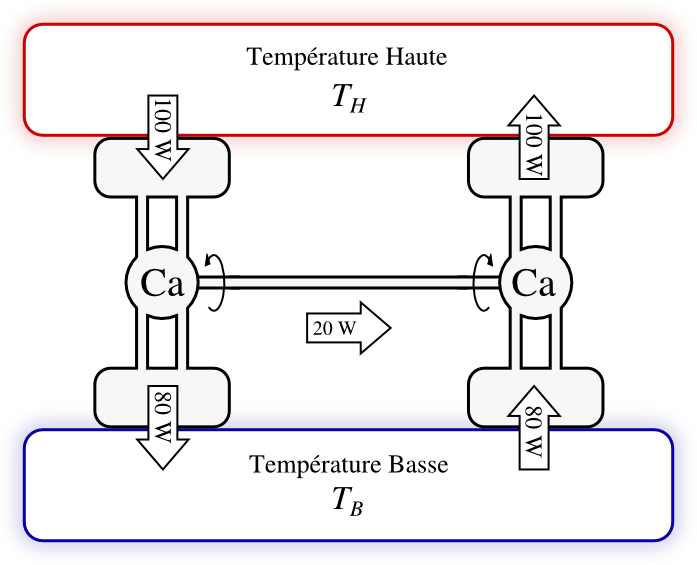
\includegraphics[height=8cm]{images/carnot_moteur_refrigerateur.png}
			\end{center}
			\supercaption{Deux machines de Carnot, un moteur (à gauche) et un réfrigérateur (à droite). La première alimente la seconde, et comme elles sont réversibles, les flux de chaleur sont compensés.}{schéma \cczero \oc}
			\label{fig_deux_machines_de_carnot}
		\end{figure}

		Pourquoi une telle machine serait-elle la plus efficace que l’on puisse concevoir ? On peut montrer par l’absurde qu’un moteur ayant une efficacité \emph{supérieure} à un moteur réversible ne peut exister (\cref{fig_plus_que_machine_de_carnot}). Le travail fourni par cette machine hypothétique pourrait être utilisé pour alimenter un réfrigérateur réversible. Ces deux machines réunies, ensemble, ne consommeraient alors aucun travail, mais provoqueraient tout de même un flux de chaleur depuis le réservoir froid vers le réservoir chaud. Selon Carnot, et d’après le second principe dont nous avons admis la validité, c’est impossible : une telle machine ne peut donc exister.

		\begin{figure}
			\begin{center}
				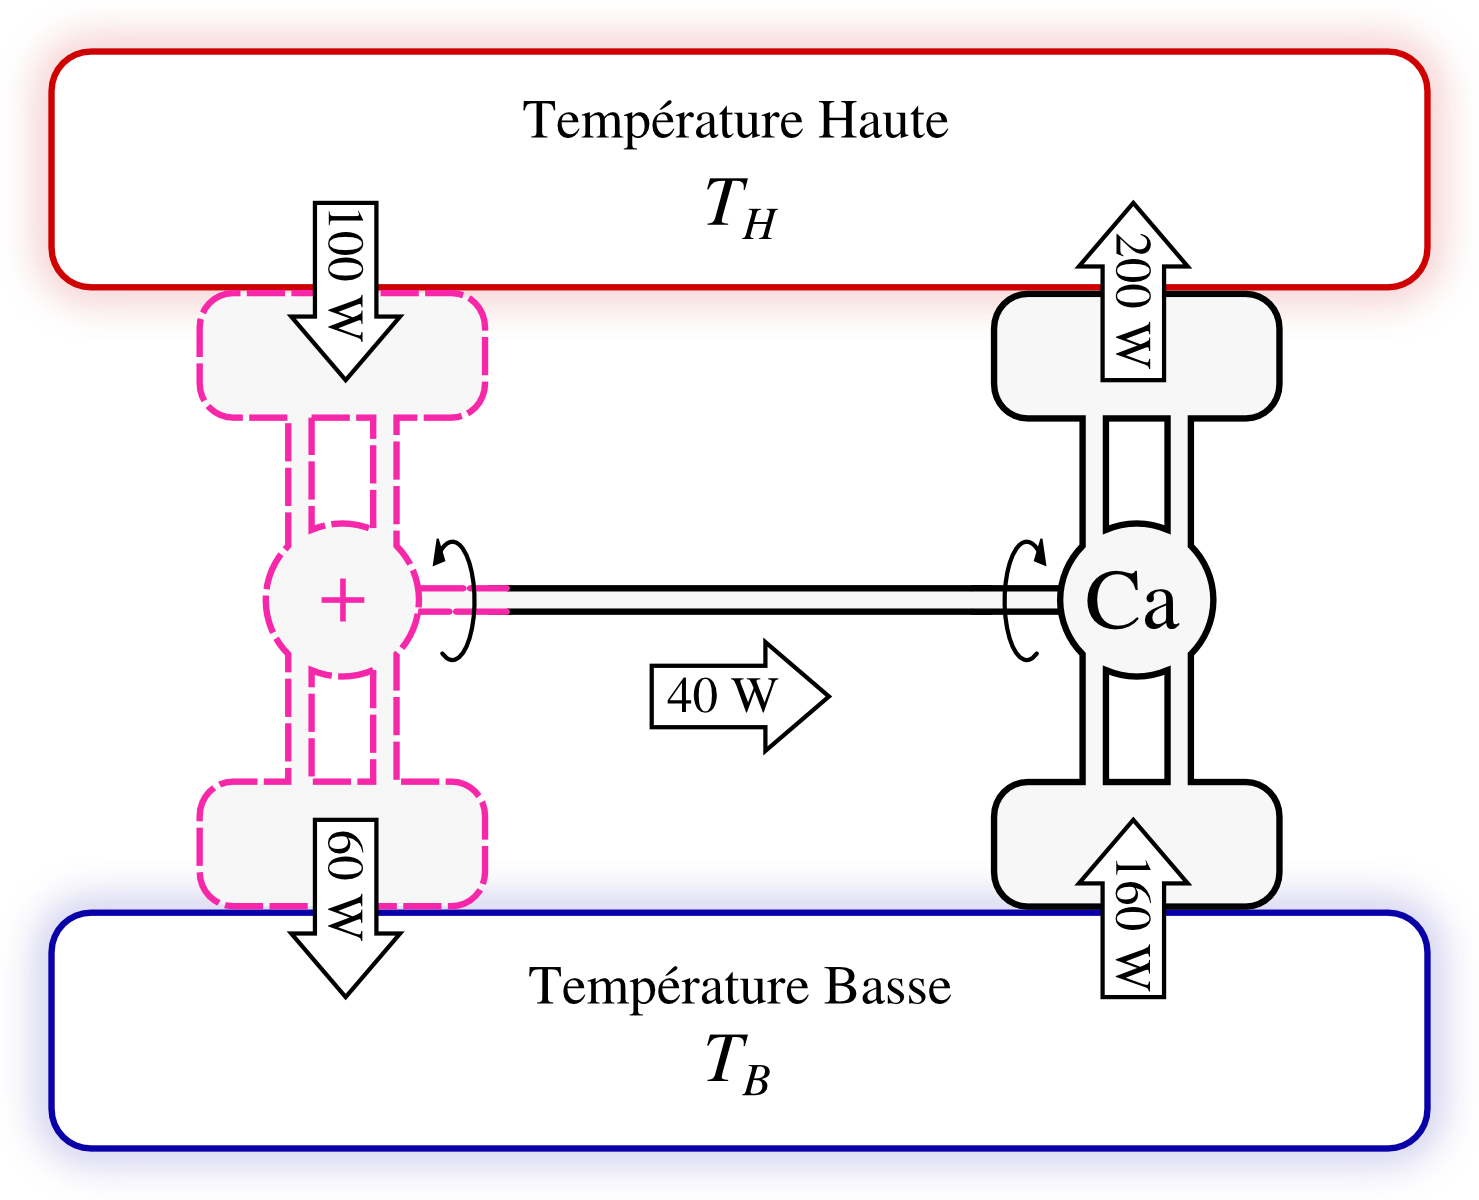
\includegraphics[height=8cm]{images/carnot_moteur_plusplus.png}
			\end{center}
			\supercaption{Démonstration par l’absurde du fait que le meilleur moteur possible est réversible.
		Un hypothétique moteur (à gauche) qui aurait une plus grande efficacité qu’un réfrigérateur réversible (à droite) pourrait simplement alimenter ce dernier. Ainsi, on obtiendrait un flux net spontané de chaleur (de~\SI{100}{\watt}) depuis la source froide vers la source chaude, sans apport net de travail : d’après le second principe, c’est impossible.}{schéma \cczero \oc}
			\label{fig_plus_que_machine_de_carnot}
		\end{figure}

		Cette méthode de raisonnement par combinaison de machines hypothétiques et théoriques, même s’il peut dérouter, est une excellente façon d’approcher la théorie des machines thermodynamiques. L’étudiant/e est vivement encouragé/e à expérimenter ainsi, en se posant par exemple les questions suivantes :

		\begin{itemize}
			\item Pourquoi le meilleur réfrigérateur possible fonctionne-t-il de façon réversible ?
			\item Pourquoi ne peut-on pas améliorer l’efficacité d’un moteur en retournant ses rejets de chaleur vers la source chaude à l’aide d’une pompe à chaleur réversible ?
		\end{itemize}


	\subsection{Élaboration du cycle de Carnot}
	\label{ch_elaboration_cycle_carnot}

		\thermoquotebegin{O}
			Mais pour tirer des machines à haute pression des résultats vraiment avantageux, il faut que la chute du calorique y soit mise à profit le mieux possible. Il ne suffit pas que la vapeur prenne naissance à une température élevée : il faut encore que par l’extension de son volume elle arrive à une température assez basse. Le caractère d’une bonne machine à vapeur doit donc être non seulement d’employer la vapeur sous une forte pression, mais \emph{de l’employer sous des pressions successives très-variables, très-différentes les unes des autres, et progressivement décroissantes}.
		\thermoquoteend{Sadi Carnot, 1824~\cite{carnot1824}}{\onlyframabook{\vspace{3em}}}%handmade
		
		Nous avons donc vu que l’efficacité maximale d’une machine est atteinte lorsque son fonctionnement est réversible. À partir de ce constat, Carnot raisonne de la façon suivante :

		\begin{enumerate}
			\item Toutes les machines thermiques fonctionnent avec la dilatation et la contraction d’un corps soumis alternativement à deux températures ;
			\item Pour qu’ils soient réversibles, c’est-à-dire pour pouvoir être effectués dans le sens inverse, tous les échanges de chaleur doivent être effectués avec des différences de température infinitésimales : ces transformations seront alors \emph{isothermes} ;
		\end{enumerate}\vspace{-0.7em}%handmade
		
		\begin{enumerate}% hack so rest of list may wrap around quote
			\shift{2}
			\item Pour qu’elles soient réversibles, les phases où le corps change de température (pour passer d’un réservoir de chaleur à un autre) doivent se faire sans échange de chaleur : ces transformations seront alors \emph{adiabatiques}.
			\item Pour permettre un retour en arrière avec chaque évolution, il faut qu’elles soient toutes \emph{réversibles} (infiniment lentes).
		\end{enumerate}

		L’essentiel est dit. Carnot vient ici de dessiner un cycle thermodynamique théorique, composé de deux évolutions isothermes et deux évolutions adiabatiques. Il n’a pas eu besoin de quantifier le moindre transfert ; et ne s’est pas encore soucié du moindre détail technologique. Pourtant, il est certain que le cycle thermodynamique qu’il décrit est le plus efficace --\ le moins inefficace !\ -- qu’il soit possible d’effectuer.
		 

	\subsection{Les quatre étapes du moteur de Carnot}
	\label{ch_descritpion_cycle_carnot}

		Nous pouvons décrire le \vocab{cycle de Carnot} avec une quantité de masse prisonnière dans un cylindre à laquelle l’on fait subir quatre transformations (\cref{fig_carnot_quatre_etapes}). Elle évolue ainsi entre les températures $T_H$ (source «~chaude~» à haute température) et~$T_B$ (source «~froide~» à basse température), pour développer un travail net :

		\begin{itemize}

			%renewing bullet as an image at every \item. Quite a lousy hack, no doubt.
			\renewcommand\labelitemi{
\includegraphics[width=3cm]{images/illustration_adiabatique.png}}
			\onlyframabook{\setlength{\itemindent}{2.2cm}}
			\renewcommand\itemsep{1cm}
			\renewcommand\topsep{3cm}

			\item \textbf{Compression adiabatique réversible de 1 à 2}

				Dans cette étape, nous souhaitons amener le fluide jusqu’à une haute température sans lui apporter de chaleur. 
				
				Le cycle débute en 1, lorsque le fluide est dans le cylindre à température basse~$T_B$. 

				Pour l’amener à température haute (et ainsi permettre un transfert de chaleur réversible en phase $2\to3$), le fluide est compressé de façon adiabatique réversible (\S\ref{ch_gp_isentropiques} \& \S\ref{ch_lv_isentropiques}). La température du fluide augmente de~$T_B$ à~$T_H$.

				Cette phase est \emph{consommatrice} de travail ($W_{1 \to 2} > 0$).

			% again
			\renewcommand\labelitemi{
\includegraphics[width=3cm]{images/illustration_th.png}}
			\item \textbf{Chauffage isotherme de 2 à 3}
				
				Dans cette étape, nous souhaitons capter une quantité $Q_{TH}$ de chaleur de la source à haute température.

				En 2, le fluide se trouve compressé dans le piston, à la température $T_H$. Le cylindre est mis au contact de la source chaude (température $T_H$) et on fournit de la chaleur avec une différence de température infinitésimale : c’est une détente isotherme(\S\ref{ch_gp_isothermes} \& \S\ref{ch_lv_isothermes}). La température du fluide reste constante à~$T_H$.

				Cette phase est productrice de travail ($W_{2 \to 3} < 0$). 

			% Baby one more time
			\renewcommand\labelitemi{
\includegraphics[width=3cm]{images/illustration_adiabatique.png}}
			\item \textbf{Détente adiabatique de 3 à 4}

				Dans cette étape, nous souhaitons faire chuter la température du fluide jusqu’à celle de la source froide ($T_B$). 

				En 3, le fluide se trouve toujours à température $T_H$. Le cylindre est alors isolé thermiquement et le fluide est détendu de façon à extraire du travail et réduire sa température sans transfert de chaleur : c’est une détente détente adiabatique réversible. Le piston poursuit son lent recul, et la température du fluide descend jusqu’à~$T_B$. 

				Cette phase est productrice de travail ($W_{3 \to 4} < 0$).

			% one last time
			\renewcommand\labelitemi{
\includegraphics[width=3cm]{images/illustration_tb.png}}
			\item \textbf{Refroidissement isotherme de 4 à~1}

				Dans cette dernière étape, nous souhaitons rejeter une quantité $Q_{TB}$ de chaleur dans le puits à basse température.
				
				En 4, le fluide est à température basse $T_B$. Pour le ramener à son volume initial, il faut lui retirer de la chaleur. Nous procédons à un refroidissement isotherme : le piston est avancé progressivement, et la température du fluide est maintenue constante à~$T_B$.

				Cette phase est consommatrice de travail ($W_{4 \to 1} > 0$).

		\end{itemize}

		Au final, le moteur a reçu une quantité de chaleur $|Q_{TH}|$ à haute température, et rejeté une quantité $|Q_{TB}|$ plus faible à basse température. La différence entre ces deux quantités est le travail produit, $W_\net = W_{1 \to 2} + W_{2 \to 3} + W_{3 \to 4} + W_{4 \to 1} = - Q_{TH} - Q_{TB}$ (\ref{def_travail_net}).
		
		Cette quantité de travail $W_\net$ représente le maximum qu’il soit possible d’obtenir à partir d’une quantité de chaleur $Q_{TH}$, entre deux températures données~$T_B$ et~$T_H$. 

		\begin{landscape}

		\begin{figure}
			\begin{center}
				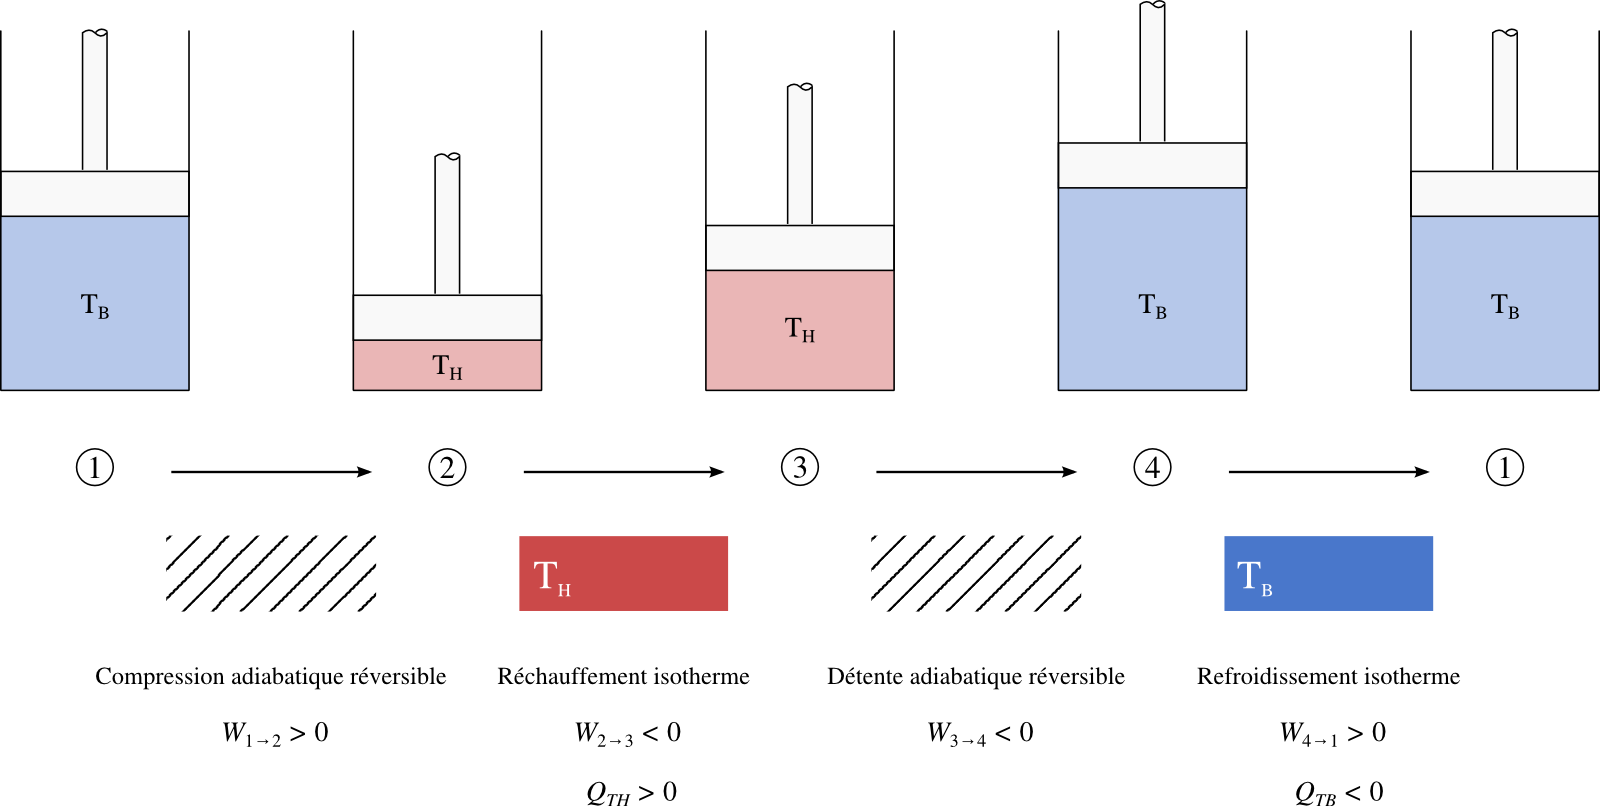
\includegraphics[width=\linewidth]{images/moteur_carnot_sf.png}
			\end{center}
			\supercaption{Les quatre étapes du moteur de Carnot, réalisées avec une quantité de masse fixe en les séparant dans le temps. Le cycle est tel que lorsqu’elles sont effectuées dans l’ordre inverse ($1 \to 4 \to 3 \to 2 \to 1$), les transferts sont exactement opposés.}{schéma \cczero \oc}
			\label{fig_carnot_quatre_etapes}
		\end{figure}

		\begin{figure}
			\begin{center}
				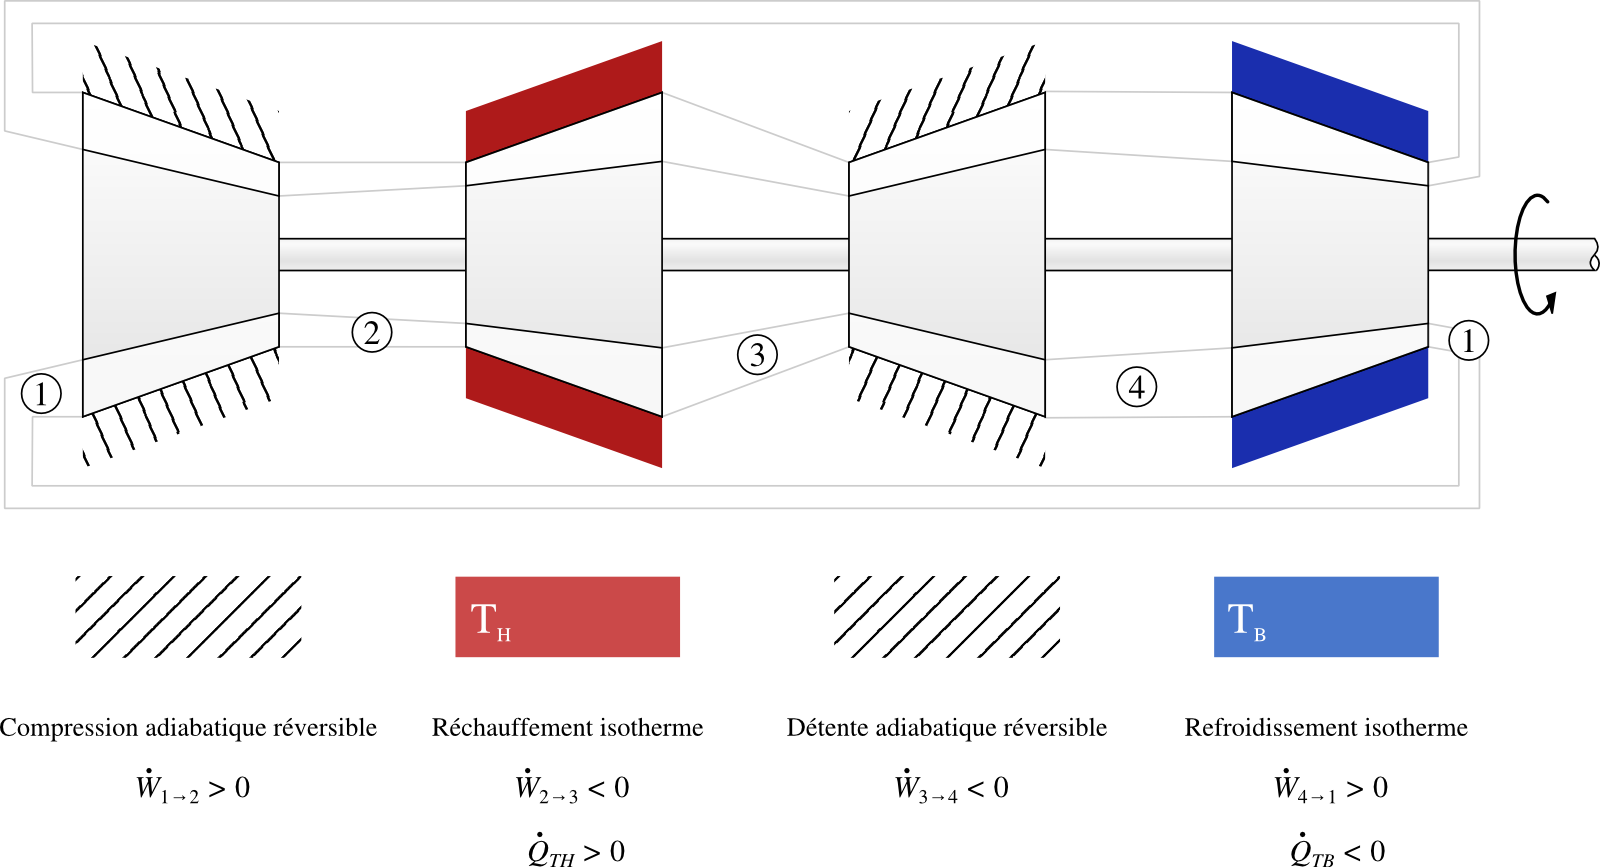
\includegraphics[width=\linewidth]{images/moteur_carnot_so.png}
			\end{center}
			\supercaption{Les quatre étapes du moteur de Carnot, réalisées avec un débit de masse constant en les séparant dans l’espace. Ici encore, le cycle est tel que lorsque le sens de circulation est inversé (devenant $1 \to 4 \to 3 \to 2 \to 1$), les transferts sont exactement opposés.}{schéma \ccbysa \olivier}
			\label{fig_carnot_quatre_etapes_so}
		\end{figure}

		\end{landscape}


		Le cycle du moteur de Carnot peut être tracé sur un diagramme pression-volume (comme par exemple en \cref{fig_p-v_gp_carnot} avec un gaz parfait). On observe notamment que les phases de compression se déroulent à une pression et un volume plus bas que les phases de détente : le cycle est producteur de travail. Comme toutes les évolutions sont réversibles, l’aire circonscrite dans le parcours 1-2-3-4-1 représente la quantité de travail net $W_\net$ produite.

		\begin{figure}[htc]%handmade
			\begin{center}
				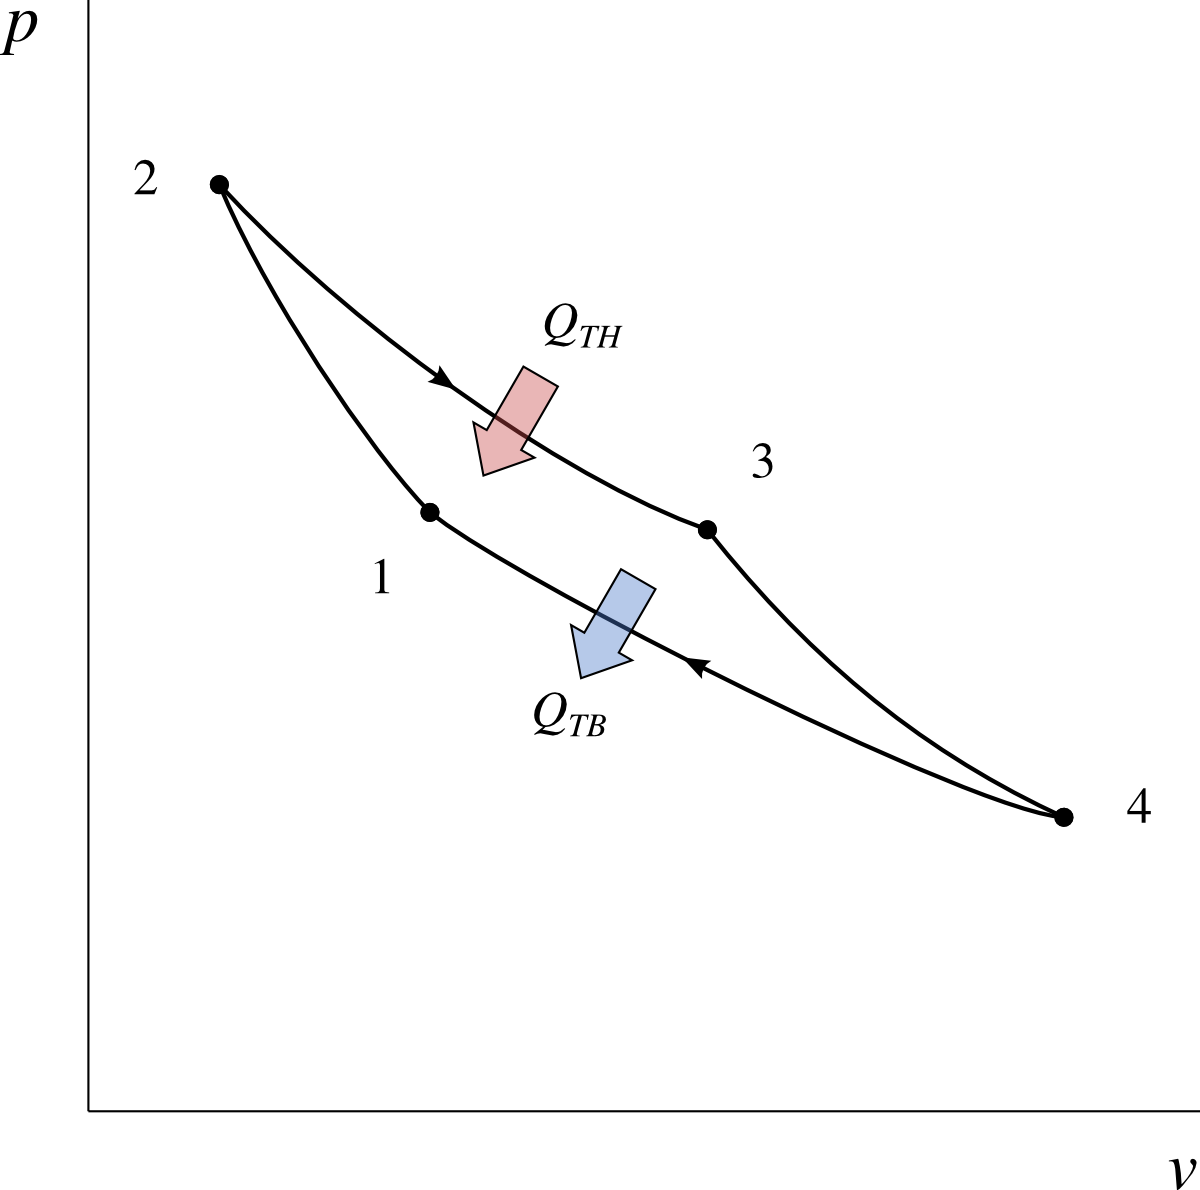
\includegraphics[width=\didacticpvdiagramwidth]{images/carnot_pv_gp_moteur.png}
			\end{center}
			\supercaption{Diagramme pression-volume du moteur de Carnot réalisé avec un gaz parfait. Les évolutions $2\to 3$ et $4\to 1$ se font respectivement à $T_H$ et $T_B$.}{schéma \cczero \oc}
			\label{fig_p-v_gp_carnot}
		\end{figure}

		\thermoquotebegin{O}
			Pour utiliser complètement la force motrice dont on peut disposer, il faudrait que la détente fût poussée jusqu’à ce que la température de la vapeur se réduisît à celle du condenseur; mais des considérations pratiques tirées de la manière dont on utilise dans les arts la force motrice du feu, s’opposent à ce que l’on atteigne cette limite.
		\thermoquoteend{Émile Clapeyron, 1834~\cite{clapeyron1834}}{}

		Le fait qu’aucune de ces étapes ne soit réalisable en pratique n’aura pas échappé à l’étudiant/e perspicace : pour que toutes ces phases soient réversibles, il faut que le mouvement du piston soit infiniment lent, et qu'ainsi le fluide parcoure le cycle en une durée de temps infinie. Le moteur de Carnot atteint donc l’efficacité maximale avec une puissance infiniment faible.
		
		\begin{anexample}
		\label{ex_cycle_carnot}
			On effectue un cycle de Carnot entre les températures de~\SI{600}{\degreeCelsius} et~\SI{100}{\degreeCelsius}. On utilise~\SI{100}{\gram} d’air prisonnier dans un cylindre, à pression de \SI{1}{\bar}. Quel est le travail à investir ? Quel est le travail récupéré ? Quel est le rendement ?
				 \begin{answer}
				 	Nous commençons par faire monter la température jusqu’à~\SI{600}{\degreeCelsius}, avec une évolution adiabatique réversible ($1\to 2$). Le coût énergétique pour cela sera $w_{1\to 2} = c_v \ \Delta T = \num{1005}\times(\num{600}-\num{100}) = \SI{+502,5}{\kilo\joule\per\kilogram}$ (\ref{eq_gp_travail_isentropique_sf}) et $q_{1\to 2} = 0$ . L’\cref{eq_isentropique_horrible2} nous apporte la pression finale : $p_2 
				 	= p_1 \left(\frac{T_2}{T_1}\right)^{\frac{\gamma}{\gamma - 1}} 
				 	= 1 \times \left(\frac{\num{600}\plustwoseventhree}{\num{100}\plustwoseventhree}\right)^{\frac{\num{1,4}}{\num{1,4} - 1}}
				 	= \SI{19,6}{\bar}$.
				 		\begin{remark}Cette phase a pour seul but de faire monter la température de façon à pouvoir ensuite capter la chaleur sans irréversibilité, ce qui arriverait si le gaz était chauffé à une température inférieure à~\SI{600}{\degreeCelsius}.\end{remark}
					Nous pouvons maintenant capter de la chaleur à température constante ($2 \to 3$). Nous choisissons de détendre le gaz jusqu’à~$p_3 = \SI{4}{\bar}$. Ainsi le transfert de chaleur est de $q_{2 \to 3} 
					= - R \ T_2 \ln\left(\frac{p_3}{p_2}\right)
					= - \num{287} \times (600\plustwoseventhree) \times \ln \left(\frac{4}{\num{19,6}}\right)
					= \SI{398,2}{\kilo\joule\per\kilogram}$ (\ref{eq_gp_travail_isotherme_sf2}, une réception par le gaz) et le travail est de $w_{2 \to 3} = - q_{2 \to 3} = \SI{-398,2}{\kilo\joule\per\kilogram}$ (\ref{eq_gp_chaleur_isotherme_sf}, une perte par le gaz).
						\begin{remark}Promesse tenue : nous avions étudié les transformations isothermes aux sections \S\ref{ch_gp_isothermes} et \S\ref{ch_lv_isothermes} précisément pour pouvoir nous en servir ici…\end{remark}
				 		\begin{remark}Le choix de la pression $p_3$ ou de son volume correspondant $v_3$ est entièrement arbitraire et il n’affecte aucun des résultats obtenus ici.\end{remark}
				 	Nous procédons à la détente du gaz, de façon à récupérer autant de travail que possible et à faire chuter sa température ($3 \to 4$). L’évolution est adiabatique réversible, ainsi $w_{3\to 4} = c_v \ \Delta T = -w_{1\to 2} = \SI{-502,5}{\joule\per\kilogram}$ et $q_{3\to 4} = 0$. Avec l’\cref{eq_isentropique_horrible2} nous obtenons la pression finale : $p_4 = p_3 \left(\frac{T_4}{T_3}\right)^{\frac{\gamma}{\gamma - 1}} = \SI{0,2}{\bar}$.
				 		\begin{remark}Le travail récupéré de~3 à~4 est exactement opposé à celui investi de~1 à~2. Dans un cycle de Carnot, c’est pendant les transferts de chaleur que les travaux aboutissent à la production d’un travail net.\end{remark}
				 	Enfin, pour ramener le fluide à son état initial (\S\ref{ch_construction_cycle}), il faut refroidir le gaz ($4 \to 1$). Ce refroidissement est à température constante, ainsi  $q_{4 \to 1} 
				 	= - R \ T_4 \ln\left(\frac{p_1}{p_4}\right)
				 	= \SI{-170,2}{\kilo\joule\per\kilogram}$ (\ref{eq_gp_travail_isotherme_sf2}, une perte par le gaz) et le travail est de $w_{4 \to 1} = - q_{4 \to 1} = \SI{+170,2}{\kilo\joule\per\kilogram}$ (\ref{eq_gp_chaleur_isotherme_sf}, une réception par le gaz).
				 		\begin{remark}C’est une évolution fort complexe pour une étape si peu glorieuse : celle du rejet de la chaleur inutilisable ! Il nous faut non seulement procéder infiniment lentement avec des débattements en volumes importants, mais aussi \emph{investir} un travail considérable pour retourner en 1.\end{remark}
				 	Quel est le bilan du cycle ? Les phases de compression ont demandé $w_\text{compression} 
				 	= w_{1\to 2} + w_{4\to 1} = \SI{+672,7}{\kilo\joule\per\kilogram}$. 
				 	À la détente nous avons récupéré $w_\text{détente} 
				 	= w_{2\to 3} + w_{3\to 4} = \SI{900,7}{\kilo\joule\per\kilogram}$. 
				 	Le travail net est de $w_\net 
				 	= w_\text{compression} + w_\text{détente} = \SI{-228}{\kilo\joule\per\kilogram}$ ;
				 	$W_\net = m \ w_\net = \SI{-22,8}{\kilo\joule}$. 
				 		\begin{remark}Nous avons pris la masse de gaz en compte le plus tard possible. Si nous avions étudié un cycle réalisé en continu comme représenté en \cref{fig_carnot_quatre_etapes_so}, il nous suffirait de remplacer et $m$ par $\dot m$ pour obtenir les puissances recherchées en \si{watts}.\end{remark}
				 		\begin{remark}Il faut investir beaucoup de travail par rapport à la quantité reçue en retour, ce qui est une caractéristique plutôt indésirable que nous quantifierons au \coursdix sous le nom de \vocab{marge de travail} (\ref{eq_marge_travail}).\end{remark}
				 	Le rendement (\ref{def_rendement_moteur}), enfin, est de $\eta_\text{moteur} 
				 	= \left|\frac{w_\net}{q_\inn}\right| 
				 	= -\frac{w_\net}{q_{2 \to 3}} 
				 	= -\frac{\num{-228}}{\num{398,2}} = \SI{57,3}{\percent}$.
				 		\begin{remark}Bien que le cycle soit déjà irréalisable en pratique, ce maigre rendement est le plus grand qu’il soit physiquement possible d’atteindre entre les deux températures~\SI{600}{\degreeCelsius} et~\SI{100}{\degreeCelsius}.\end{remark}
				 		\begin{remark}Nous aurions aussi pu effectuer ces calculs en utilisant un liquide/vapeur au lieu d’air : cela n’aurait pas modifié les résultats finaux.\end{remark}
				 \end{answer}
		\end{anexample}
		

	\subsection{Quatre étapes ou quatre temps ?}
	
		Les moteurs à pistons sont souvent classés selon leur mode de fonctionnement. Les moteurs à \vocab{deux temps} effectuent une détente par tour de vilebrequin (tous les deux mouvements de piston) ; tandis que les moteurs à \vocab{quatre temps} effectuent une détente tous les deux tours. La distinction porte sur le mode de vidange des gaz brûlés et de leur remplacement par de l’air frais.
		
		La transposition du moteur de Carnot à la réalité, dans laquelle il faudra éventuellement vidanger le fluide ou le transvaser dans un cylindre séparé pour son refroidissement, pourra se faire avec deux ou quatre temps au choix de l’ingénieur/e. Ainsi ne peut-on pas associer le cycle de Carnot, même s’il est bien constitué de quatre \emph{étapes}, à l’un ou l’autre de ces deux modes de fonctionnement en particulier.
		

	\subsection{Le réfrigérateur de Carnot}

		En inversant le sens de fonctionnement du moteur décrit plus haut, on crée un réfrigérateur, un climatiseur, ou une pompe à chaleur de même efficacité. Le fluide passe alors par les mêmes états, mais en parcourant le chemin inverse (1-4-3-2-1) comme montré en \cref{fig_p-v_gp_carnot_inversé}. La chaleur $Q_{TB} > 0$ est \emph{captée} de la source froide, le travail $W_\net > 0$ est \emph{reçu} par la machine, et la chaleur $Q_{TH} < 0$ est rejetée par la machine vers la source à haute température.

		Ce cycle permet d’obtenir le rendement maximal (le «~moins mauvais~» rendement, car il n’est pas infini) d’un système de climatisation ou d’une pompe à chaleur fonctionnant entre deux températures $T_H$ et $T_B$ données.

		\begin{figure}
			\begin{center}
				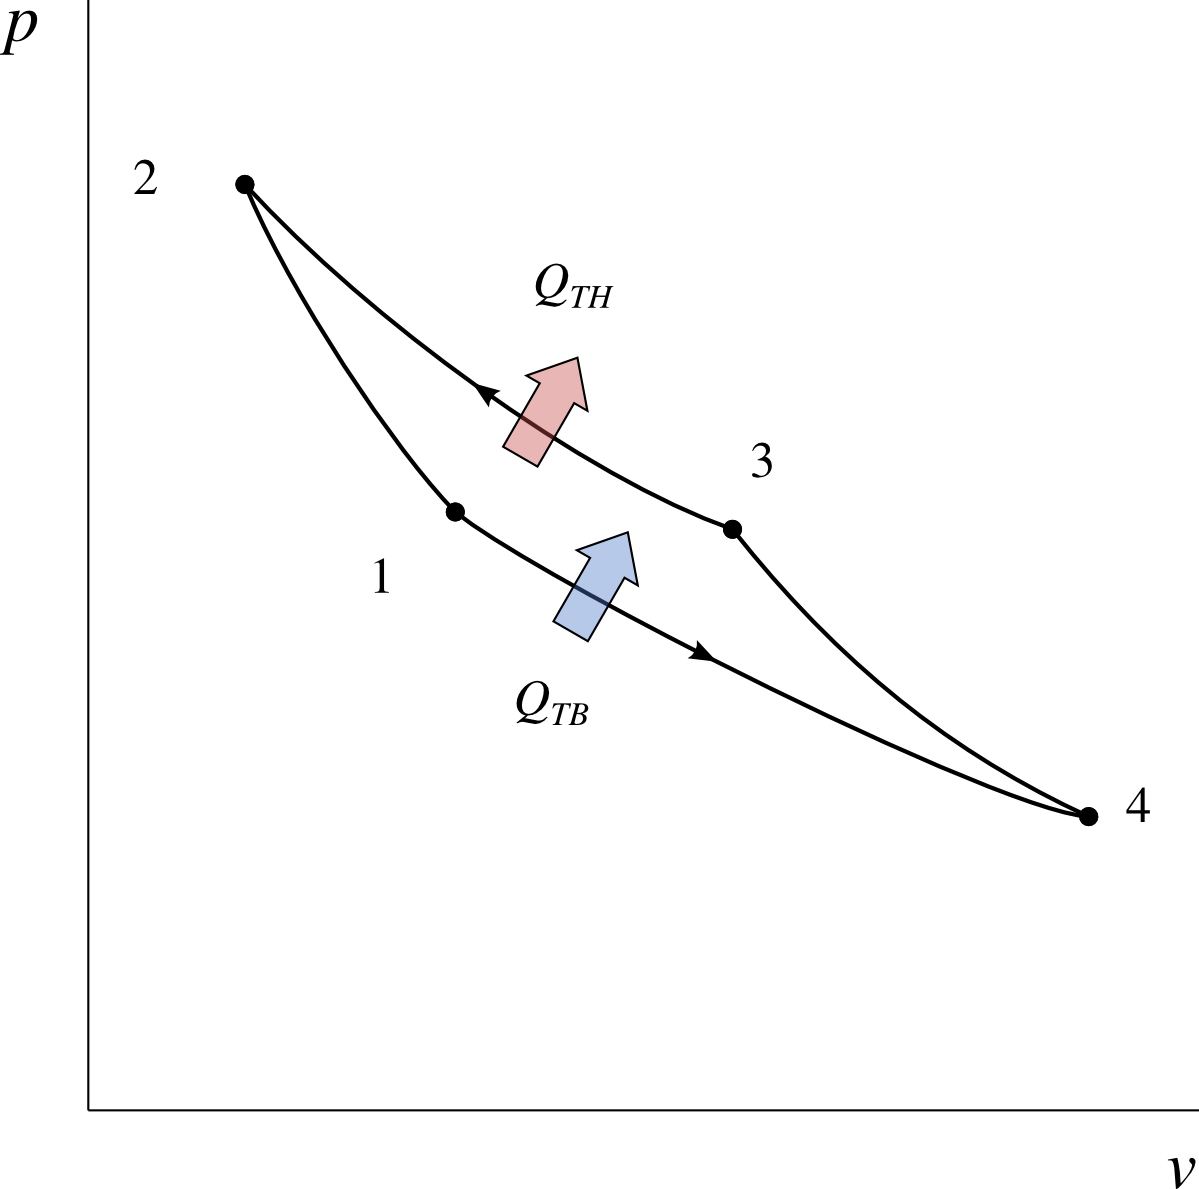
\includegraphics[width=\didacticpvdiagramwidth]{images/carnot_pv_gp_refrigerateur.png}
			\end{center}
			\supercaption{Diagramme pression-volume pour un cycle de Carnot inversé, c’est-à-dire en mode de réfrigération (réfrigérateur ou pompe à chaleur), avec un gaz parfait.}{schéma \cczero \oc}
			\label{fig_p-v_gp_carnot_inversé}
		\end{figure}


\section{L’échelle de température thermodynamique}


	\subsection{L’essentiel à retenir}
	
		Kelvin définit une échelle de température, dite de \vocab{température absolue}. À l’intérieur d’une machine de Carnot, le rapport des températures maximale $T_H$ et minimale $T_B$ est défini comme égal au rapport des débits sous forme de chaleur, c’est-à-dire :
		\begin{equation}
			\left| \frac{\dot Q_{TH}}{\dot Q_{TB}} \right| \equiv  \frac{T_H}{T_\B } \tag{\ref{def_échelle_température_kelvin}}
		\end{equation}
		\begin{equationterms}
			\item par définition, dans une machine de Carnot,
			\item où \tab $\dot Q_{TH}$ \tab est le débit de chaleur absorbé ou rejeté à haute température ($\dot Q_{TB}$, à basse température),
			\item et où les températures sont absolues (mesurées en \si{\kelvin}).
		\end{equationterms}

		Cette \cref{def_échelle_température_kelvin} est une définition. On peut donc déterminer la température d’un corps sans devoir utiliser un fluide en particulier. Kelvin étalonne son échelle de sorte que $\SI{0}{\degreeCelsius} = \SI{273,15}{\kelvin}$. 
		
		Les paragraphes qui suivent détaillent le cheminement qui a mené à cette définition. Ils sont destinés aux lecteurs curieux, et peuvent être survolés sans danger par l’étudiant/e ou l’ingénieur/e pressé/e. 


	\subsection{Qu’est-ce qu’une échelle en physique ?}
	
		Pour quantifier une propriété en physique (par exemple, quantifier «~la masse~» ou «~la couleur~»), il faut avoir défini trois choses :
		
		\begin{description}
			\item [Un degré zéro] qui définit ce que représente zéro propriété (zéro masse, zéro pression, etc.) ;
			\item [Un étalon] arbitraire qui sert de calibre (par exemple, un objet de masse une livre, de longueur un mètre) ;
			\item [Une échelle] qui permet de \emph{définir} la propriété entre le degré zéro et l’étalon (par exemple, ce qu’est «~deux fois plus~» ou «~deux fois moins~» de masse, de lumière, etc.).
		\end{description}


	\subsection{Les limites des thermomètres de Celsius et Fahrenheit}
	\label{thermometres_celsius_fahrenheit}
	
		Au début du \textsc{xix}\ieme siècle, les deux échelles de température que nous utilisons aujourd’hui dans la vie courante, celles du suédois \wf{Anders Celsius} et de l’allemand \wf{Gabriel Fahrenheit}, sont déjà en usage. Qu’en est-il de ces deux échelles d’un point de vue physique ?
			
		\begin{itemize}
			\item Le degré zéro est plutôt facile à définir (c’est le point où les corps sont entièrement figés, incapables de fournir de la chaleur) mais ni Fahrenheit ni Celsius ne sont capables de le situer avec certitude ;
			\item Les étalons de Celsius et Fahrenheit sont sensiblement différents. Celsius choisit le gel de l’eau pure, Fahrenheit de l’eau salée, à pression atmosphérique, et lui attribuent chacun la graduation relative «~zéro~».
			\item Les échelles de Celsius et Fahrenheit, en revanche, sont strictement identiques. En effet, pour \emph{mesurer} les températures autour de leurs étalons, les deux scientifiques mesurent la contraction et la dilatation d’un liquide dans un tube. Entre son zéro et l’ébullition de l’eau à pression atmosphérique, Celsius trace 100 graduations%
			\footnote{En fait, Celsius utilise initialement une échelle inversée, allant de~\SI{100}{\celsius} au gel jusqu’à~\SI{0}{\celsius} à l’ébullition !} ; Fahrenheit, 212 graduations%
			\footnote{Cette graduation est probablement choisie pour se recaler facilement sur sa \emph{première} graduation, étalonnée sur le gel de l’eau pure (32) et la température du corps humain (96). Des étalons fort difficiles à reproduire !}.
		\end{itemize}
		
		Le principal problème avec ces deux échelles est que la température n’est bien définie que dans le domaine d’existence des thermomètres à liquide. Quel que soit le fluide utilisé (mercure, alcool, eau), il finit toujours par geler ou bouillir quelque part ; et les graduations ne donnent alors plus d’information utile. Par exemple, Celsius ne peut pas \emph{définir} ou même décrire ce qui permet de reconnaître une température de~\SI{1200}{\celsius}.
		
		En plus de cela, les deux échelles sont peu intuitives à utiliser en dessous du gel de l’eau. Pour peu que l’on admette, par exemple, que \SI{40}{\celsius} puisse être «~deux fois plus de température~» que \SI{20}{\celsius}, alors à quoi correspondrait une température deux fois plus haute que \SI{-10}{\celsius} ?\footnote{Cela revient à poser la question : peut-on écrire $\frac{\SI{40}{\celsius}}{\SI{20}{\celsius}}$ et est-ce égal à $\frac{\SI{80}{\celsius}}{\SI{40}{\celsius}}$ ? La réponse moderne à cette question est non.}
		
	
	\subsection{Le thermomètre de William Thomson}
	
		\wfd{William Thomson (Lord Kelvin)}{William Thomson}, ingénieur et physicien écossais, a bien compris ces limites. Il va proposer une échelle de température qui, elle, ne dépend pas du comportement d’un fluide dans un tube.

		Thomson s’intéresse de près au cycle de Carnot et il raisonne de la façon suivante : La seule propriété qui confère l’efficacité maximale au moteur de Carnot est le fait qu’il soit réversible. Autrement dit, toutes les machines fondées sur ce cycle et opérant entre deux températures données auront la même efficacité —\ quels que soient leur carburant, leur cylindrée, leur configuration, ou leur puissance\footnote{On pourrait par exemple «~allonger~» tant qu’on veut les phases de détente isotherme : rien ne fixe \textit{a~priori} l’état 3 décrit en \cref{fig_carnot_quatre_etapes}).}. On pourrait donc se servir de l’efficacité d’un moteur de Carnot comme mesure de la température.
		
		\thermoquotebegin{O}
			Les valeurs absolues de deux températures sont l’une par rapport à l’autre en proportion de la chaleur reçue à la chaleur rejetée dans un moteur thermo-dynamique parfait travaillant avec une source et un refroidisseur aux plus haute et basse températures respectivement.
		\thermoquoteend{William Thomson, 1854~\cite{kelvin1854}}{}
		La proposition de Thomson est la suivante : soit un corps à une température~$T_1$ (par exemple de mille unités, comme montré en \cref{fig_échelle_température_kelvin}). On y attache un moteur de Carnot, qui va fournir du travail et rejeter de la chaleur à température plus basse $T_2$. Cette température $T_2$ est deux fois plus faible que $T_1$ si le moteur rejette la moitié de la chaleur qu’il reçoit ; elle est quatre fois plus faible lorsqu’il en rejette le quart, etc. En termes mathématiques, Thomson propose\footnote{En fait, ce n’est pas si simple. Thomson propose d’abord (en 1848 \cite{kelvin1848}) une échelle dans laquelle $\frac{\dot Q_{TH}}{\dot Q_{TB}}$ est proportionnel à la \emph{différence} des températures ; ce qui en fait une échelle logarithmique de notre point de vue actuel. Il se ravise avec l’aide de James Prescott Joule pour obtenir la proposition~\ref{def_échelle_température_kelvin} six ans plus tard~\cite{kelvinjoule1854}.} :
		\begin{equation}
			\left| \frac{\dot Q_{TH}}{\dot Q_{TB}} \right| \equiv  \frac{T_H}{T_\B }
			\label{def_échelle_température_kelvin}
		\end{equation}
		\begin{equationterms}
			\item dans une machine de Carnot (en fait, pour toute machine effectuant une transformation réversible),
			\item où \tab $\dot Q_{TH}$ \tab est le débit de chaleur absorbé ou rejeté à haute température ($\dot Q_{TB}$, à basse température),
			\item et où les températures sont \vocab{absolues} (mesurées en \si{\kelvin}).
		\end{equationterms}

		\begin{figure}
			\begin{center}
				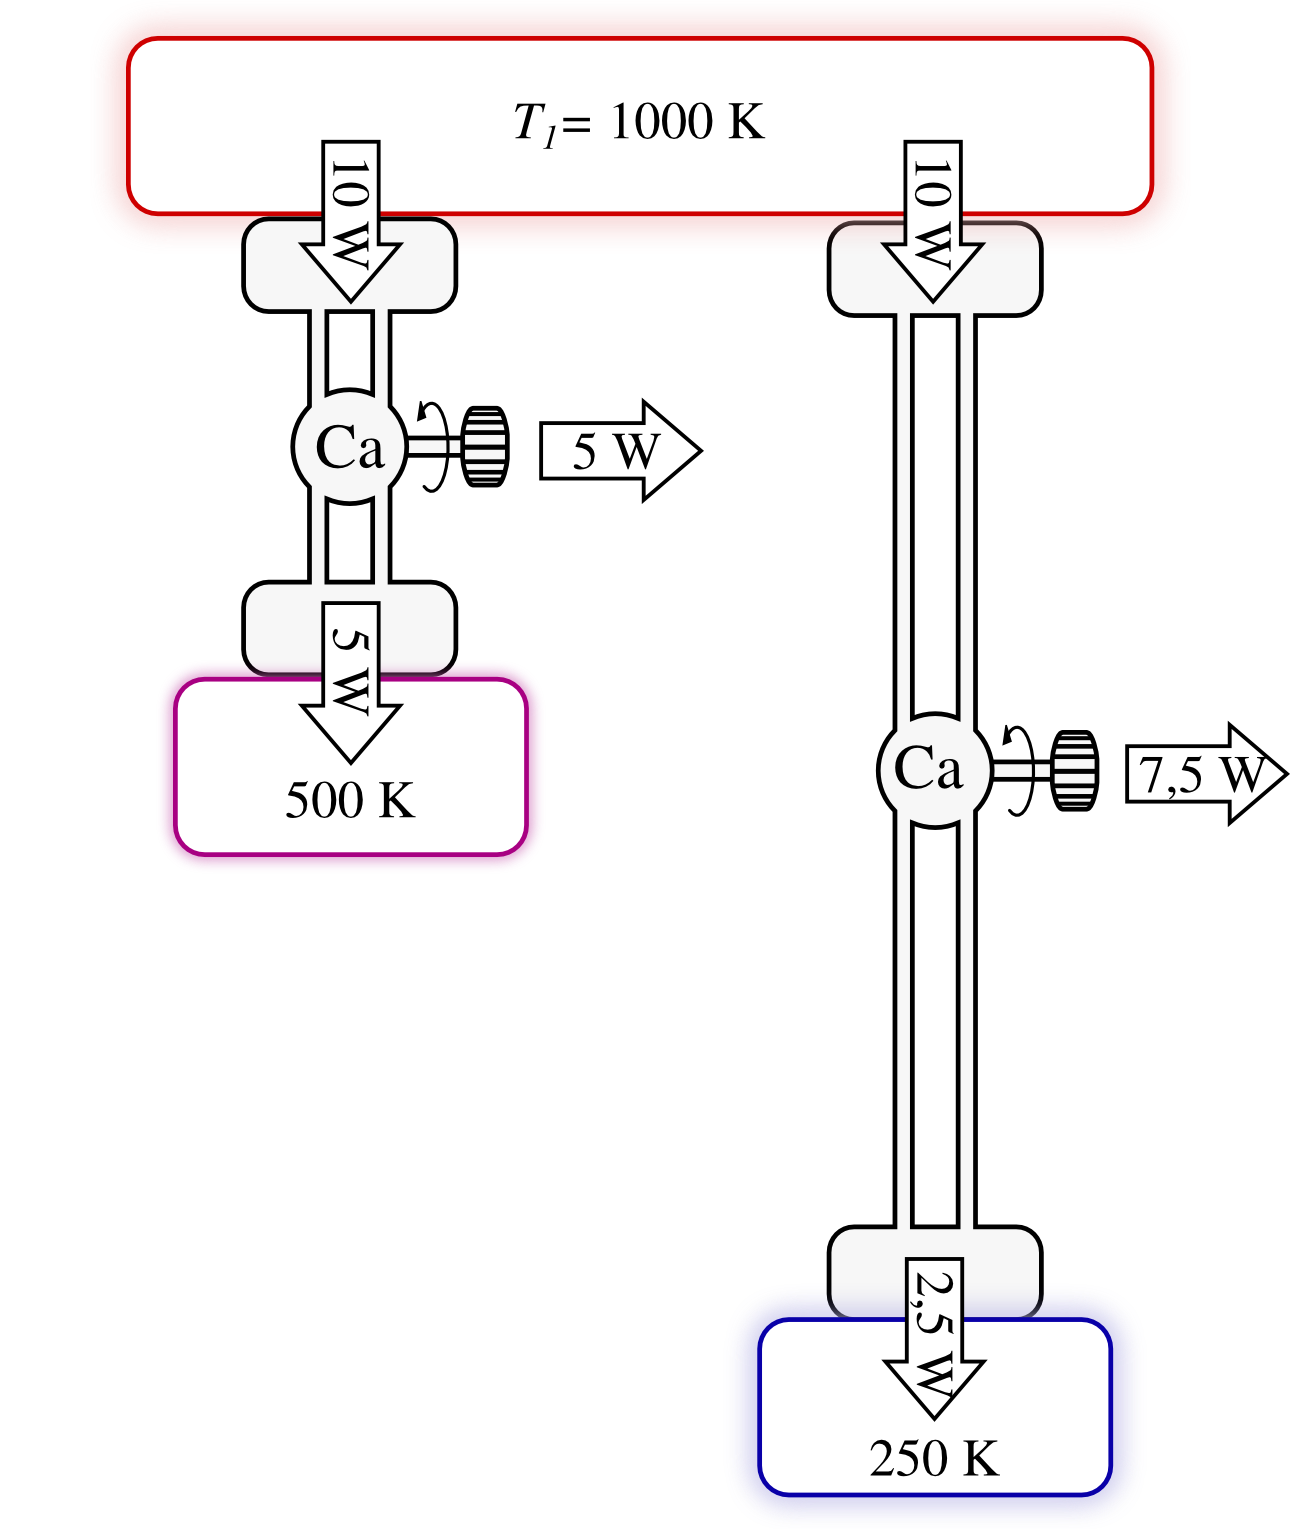
\includegraphics[width=10cm]{images/echelle_temperature_kelvin.png}
			\end{center}
			\supercaption{Expérience permettant d’illustrer l’échelle de température absolue proposée par William Thomson. Un moteur de Carnot fonctionnant entre \SI{1000}{\kelvin} et~\SI{500}{\kelvin} rejette $\frac{\num{1000}}{\num{500}} = \SI{50}{\percent}$ de la chaleur qu’il reçoit. Si la température basse est quatre fois plus faible, ce rejet est quatre fois plus faible ($\frac{\num{1000}}{\num{250}}$) que la chaleur reçue.}{}
			\label{fig_échelle_température_kelvin}
		\end{figure}

		Avec une simple manipulation des équations~\ref{def_échelle_température_kelvin} et~\ref{eq_premier_principe_machines}, on peut reformuler la définition de Kelvin comme suit :

		\begin{trucimportant}
			Soit une machine de Carnot fonctionnant 
			entre deux réservoirs thermiques séparés d’un degré de température (\SI{1}{\kelvin}),\linebreak
			et à laquelle on fournit une quantité de chaleur $Q_{H}$ de~\SI{1}{Joule} ;

			La température de la source chaude\linebreak est définie comme l’inverse du travail produit.
		\end{trucimportant}

		Les températures dans cette échelle, dite \vocab{échelle de température absolue} ou de \vocab{température thermodynamique}, sont toujours positives et varient de zéro à l’infini.
		
		
	\subsection{Zéro absolu et synchronisation des échelles}
	
		Thomson dispose donc d’une \vocab{échelle} —\ une méthode permettant de définir une température «~deux fois plus élevée~».
		
		Le zéro de cette échelle correspond bien au degré zéro de température, puisqu’avec l’expérience de la \cref{fig_échelle_température_kelvin} on dispose alors d’un «~gouffre~» de température zéro qui permet de détendre les gaz jusqu’à zéro température (on peut ainsi convertir toute l’énergie interne d’un fluide en travail\footnote{On peut prendre une machine de Carnot avec $T_\B = \SI{0}{\kelvin}$. Le transfert de chaleur à la source froide est alors inutile puisque l’on a effectué une détente infinie ($3 \to 4$) pour obtenir une température de zéro. $Q_{TB}$ est alors nul, et on retrouve bien un rendement de~\SI{100}{\percent}.}).
		
		\thermoquotebegin{O}
			Cette convention particulière est que la différence de température entre les points de gel et d’ébullition de l’eau sous atmosphère standard est appelée 100 degrés.
		\thermoquoteend{William Thomson, 1854~\cite{kelvin1854}}{\onlyframabook{\vspace{1em}}}%handmade

		Reste le choix d’un étalon. Thomson revient au thermomètre de Celsius et prend le même point de référence (le gel de l’eau pure à pression atmosphérique). Observant que la contraction et la dilatation des fluides reste proportionnelle à leur variation de température absolue, il attribue à ce point de référence une valeur qui permet de conserver la même graduation thermométrique que Celsius. Pour cela, il faut que les températures \SI{100}{\celsius} et~\SI{0}{\celsius}, dont on sait qu’elles permettent un rendement maximal de~\SI{26,8}{\percent}, correspondent à des températures en \si{\kelvin} espacées de 100 unités. Le calcul est simple --\ l’étudiant/e est d’ailleurs encouragé/e à le reproduire\ -- et Thomson obtient la relation :
			\begin{equation}
			\SI{0}{\degreeCelsius} = \SI{273,15}{\kelvin}
			\label{eq_synchro_température}
			\end{equation}
		
		William Thomson, alors déjà lancé dans une carrière de scientifique époustouflante,  a trente ans lorsqu’il publie son échelle de température en 1854. En 1892 il sera sacré \textit{Premier Baron Kelvin}\footnote{On dira même \textit{The Right Honourable First Lord Kelvin of Largs, of the Order of Merit, the Royal Victorian Order, and of Her Majesty's Most Honourable Privy Council} !} ; c’est sous ce nom qu’il est connu aujourd’hui. L’unité \textit{Kelvin} (\si{\kelvin}) est officiellement attribuée à la température absolue en 1948. 
		
		Le travail de Kelvin permet donc de séparer définitivement le concept de température des fluides réels ou imaginaires comme auparavant avec l’ébullition de l’eau ou le volume des gaz parfaits (\S\ref{ch_définition_température_cours1} \& \S\ref{ch_le_manomètre_comme_thermomètre}) ; la voilà rattachée à une expérience physique précise et quantitative.

		\begin{anexample}
			Pour illustrer la nature de l’échelle de Kelvin, nous effectuons l’expérience conceptuelle suivante. Nous sommes munis d’un moteur de Carnot et d’un étalon : un bloc de titane solide que nous savons fondre à~\SI{1668}{\degreeCelsius}. Nous faisons fonctionner la machine entre la température étalon et un objet dont nous cherchons à mesurer la température. La machine absorbe~\SI{200}{\watt} et produit~\SI{45}{\watt} sous forme de travail. Quelle est la température de l’objet ?
				\begin{answer}
					Le moteur absorbe $\dot Q_\inn = \SI{200}{\watt}$, produit $\dot W_\net = \SI{-45}{\watt}$ ; il rejette donc $\dot Q_\out = - \dot Q_\inn - \dot W_\net = \SI{-155}{\watt}$. \\
					Par définition, les températures absolues sont telles qu’elles correspondent aux transferts de chaleur d’un moteur de Carnot : $\frac{T_H}{T_B} = \left|\frac{\dot Q_\inn}{\dot Q_\out}\right|$ (\ref{def_échelle_température_kelvin}). Ainsi $T_B = -\frac{\dot Q_\out}{\dot Q_\inn} T_H = -\frac{\num{-155}}{\num{200}} (\num{1668} + \num{273,15}) = \SI{1504,4}{\kelvin} = \SI{1231,2}{\degreeCelsius}$. 
				\end{answer}
					\begin{remark}On voit ici que Kelvin s’est servi de la machine de Carnot comme thermomètre. Pour en construire la graduation, il a effectué cette expérience entre les deux étalons \SI{100}{\degreeCelsius} et \SI{0}{\degreeCelsius}, et fait en sorte de les séparer par cent intervalles en unités absolues.\end{remark}
		\end{anexample}


\section{Efficacité maximale des machines}
\label{ch_efficacite_maximale_machines}
	
	La définition de la température détaillée en~\ref{def_échelle_température_kelvin} nous permet de revenir aux machines thermiques et d’apporter une réponse simple aux questions que se posait Carnot.

	\subsection{Efficacité du moteur de Carnot}
	\label{ch_efficacité_moteur_carnot}

		\thermoquotebegin{O}
			Ainsi nous sommes conduits à établir la proposition générale que voici :
\emph{La puissance motrice de la chaleur est indépendante des agens mis en œuvre pour la réaliser ; sa quantité est fixée uniquement par les températures des corps entre lesquels se fait en dernier résultat le transport du calorique}.\nolinebreak\makebox(18,5){\color{gray}\scalebox{2}{»}}\par\vspace{-0.3cm}\begin{flushright}Sadi Carnot, 1824~\cite{carnot1824}\end{flushright}
		\makebox(18,5){\color{gray}\scalebox{2}{«}}
			Notre objectif doit être toujours \emph{d’augmenter les températures et les pressions jusqu’à leurs limites pratiques les plus hautes}.
		\thermoquoteend{Rudolf Diesel, 1893~\cite{diesel1893, diesel1893en}}{}

		Lors du chapitre précédent (\S\ref{ch_rendement_moteur}), nous avons vu que le rendement d’un moteur était le rapport entre le travail produit (transfert utile, $\dot W_\net$) et la chaleur reçue (dépense énergétique, $\dot Q_\text{in}$ ). Nous avions transformé cette expression en une autre dont l’appréhension était moins facile :
		\begin{equation}
			\eta _\text{moteur} = 1 - \left| \frac{\dot Q_{TB}}{\dot Q_{TH}} \right|	\tag{\ref{eq_rendement_moteur_qin_qout}}
		\end{equation}
		\begin{equationterms}
			\item pour tout moteur thermique.
		\end{equationterms}

		Dans le cas d’une machine de Carnot, avec la relation~\ref{def_échelle_température_kelvin}, cette expression prend tout son sens en devenant :
		\begin{equation}
			\eta_\text{moteur Carnot} = 1 - \frac{T_B}{T_H}
			\label{eq_efficacité_moteur_carnot_température}
		\end{equation}
		\begin{equationterms}
			\item pour un moteur thermique réversible,
			\item et où les températures sont absolues (\si{\kelvin}).
		\end{equationterms}

		Cette expression~\ref{eq_efficacité_moteur_carnot_température} est si remarquable qu’il nous faut nous y arrêter quelques instants.

		La réponse à la question que se posait Carnot «~quelle quantité maximale de travail, en théorie, peut-on obtenir de la combustion d’une quantité donnée de charbon ?~» est ici --\ et elle est stupéfiante : \textbf{cela ne dépend que des températures haute et basse du moteur} !

		Deux remarques importantes s’imposent ici.

		\begin{itemize}
			\item Premièrement, cette efficacité n’est pas de~\SI{100}{\percent}. Pourtant, nous parlons bien ici de machines sans frottement, sans fuites, et aux mouvements infiniment lents. Par contraste, rien n’empêche un moteur électrique ou un alternateur d’atteindre une efficacité de~\SI{100}{\percent} si l’on peut s’affranchir de tous frottements. 

			Ainsi, avant même d’avoir abordé les inévitables difficultés technologiques dans la mise en place des moteurs réels, le motoriste est limité par la nature fondamentale de la chaleur dans ce qu’il peut obtenir de sa machine. Dans les chapitres suivants, nous aborderons les irréversibilités observées dans les moteurs réels, qui réduiront encore le rendement calculé ci-dessus.

			\item Secondement, cette équation est un argument fort pour augmenter la température de combustion dans les moteurs.

			En effet, en pratique la température basse~$T_B$ est bornée par celle de l’air ambiant. Le seul paramètre restant pour augmenter le rendement d’un moteur idéal est la température~$T_H$. Cette relation explique les efforts surprenants déployés par les concepteurs de moteurs pour utiliser de grandes températures (et de façon correspondante, de grandes pressions), même si les moteurs réels sont loin d’être réversibles.

		\end{itemize}

		Pour résumer, nous répondrons ainsi à la question de Carnot : plus la température à laquelle est brûlé le charbon est haute, plus la température ambiante est basse, et moins les pertes en chaleur --\ \emph{inévitables}\ -- du moteur seront grandes.
		
		\begin{anexample}
		\label{ex_efficacite_moteur_carnot}
			La température maximale atteignable dans un moteur est de \SI{600}{\degreeCelsius}, et la température à la quelle sont rejetés les gaz d’échappement est de \SI{100}{\degreeCelsius}. Quel est le rendement maximal atteignable par le moteur ?
				\begin{answer}
					Pour atteindre la conversion la plus efficace, il faudrait que le moteur soit réversible. On aurait alors, avec l’\cref{eq_efficacité_moteur_carnot_température} : $\eta_\text{moteur} = \eta_\text{moteur Carnot} = 1 - \frac{T_B}{T_H} = 1 - \frac{\num{100}\plustwoseventhree}{\num{600}\plustwoseventhree} = \SI{57,3}{\percent}$.
					\begin{remark}Attention à bien utiliser des températures absolues --\ l’erreur serait ici impardonnable.\end{remark}
					\begin{remark}Toutes les spécificités technologiques du moteur (cylindrée, méthode d’injection, etc.) peuvent éventuellement le rapprocher de ce rendement, mais jamais l’amener au delà.\end{remark}
					\begin{remark}Nous avons bien sûr retrouvé le résultat obtenu dans l’exemple \ref{ex_cycle_carnot}, avec un calcul beaucoup plus simple.\end{remark}
				\end{answer}
		\end{anexample}


	\subsection{Efficacité du réfrigérateur de Carnot}

		Nous avons vu au (\S\ref{ch_rendement_réfrigérateur}) que l’efficacité d’un réfrigérateur était la comparaison entre la chaleur extraite de la source froide (transfert utile, $\dot Q_\text{in}$ ) et le travail consommé (dépense énergétique, $\dot W_\net$).  Nous avions exprimé cette efficacité avec l’obscure expression :
		\begin{equation}
			\eta_\text{réfrigérateur} = \frac{1}{ \left| \frac{\dot Q_{TH}}{\dot Q_{TB}} \right| - 1} \tag{\ref{rendement_réfrigérateur_qin_qout}}
		\end{equation}
		\begin{equationterms}
			\item pour tout réfrigérateur.
		\end{equationterms}

		Lorsqu’il s’agit d’un réfrigérateur de Carnot, cette efficacité est fonction de la température uniquement (\ref{def_échelle_température_kelvin}) et l’on a ainsi :
		\begin{equation}
			\eta_\text{réfrigérateur Carnot} = \frac{1}{\frac{T_H}{T_B} - 1}
			\label{eq_efficacité_réfrigérateur_carnot_température}
		\end{equation}
		\begin{equationterms}
			\item pour un réfrigérateur réversible,
			\item et où les températures sont absolues (\si{\kelvin}).
		\end{equationterms}

		Les mêmes remarques que plus haut s’appliquent ici : D’une part, le rendement d’un réfrigérateur ou d’un climatiseur n’atteint jamais l’infini (un réfrigérateur de \textsc{cop} infini fonctionnerait sans apport de travail, même s’il est parfaitement isolé et doté d’un mécanisme idéal). D’autre part, cette efficacité est d’autant plus faible que la température de réfrigération $T_B$ est basse. Autrement dit, lorsque l’on refroidit un objet avec un réfrigérateur idéal, la sélection d’une température plus basse est plus coûteuse non seulement parce qu’il faut extraire plus de chaleur de l’objet, mais aussi parce que l’efficacité de l’extraction diminue. 
		 
		 \begin{anexample}
		 \label{ex_efficacite_refrigerateur_carnot}
		 	Un réfrigérateur doit amener la chambre froide à~\SI{-15}{\degreeCelsius} dans une pièce à~\SI{25}{\degreeCelsius}. Quel est le rendement maximal atteignable ?
		 		\begin{answer}
		 			L’efficacité maximale serait atteinte avec un réfrigérateur réversible, ce qui nous permettrait d’obtenir, avec l’\cref{eq_efficacité_réfrigérateur_carnot_température}, $\eta_\text{réfrigérateur} = \eta_\text{réfrigérateur Carnot} = \frac{1}{\frac{T_H}{T_B} - 1} = \frac{1}{\frac{\num{25}\plustwoseventhree}{\num{-5}\plustwoseventhree} - 1} = \num{8,94}$.
		 		\end{answer}
		 			\begin{remark}En effectuant le même calcul entre les températures \SI{185}{\degreeCelsius} et \SI{225}{\degreeCelsius}, on obtient un rendement de~\num{11,5} : celui-ci dépend non seulement de l’écart entre les températures mais aussi de leurs valeurs absolues.\end{remark}
		 \end{anexample}


	\subsection{Efficacité de la thermopompe de Carnot}

		Nous avions vu au \S\ref{ch_rendement_thermopompe} que le rendement (ou «~\textsc{cop}~») d’une pompe à chaleur est défini comme le rapport de la chaleur fournie à haute température sur le travail consommé~(\ref{def_rendement_thermopompe}). Nous avions alors transformé cette définition avec l’expression :
		\begin{equation}
			\eta_\text{thermopompe} = \frac{1}{1 - \left| \frac{\dot Q_{TB}}{\dot Q_{TH}} \right|} \tag{\ref{eq_rendement_thermopompe_qin_qout}}
		\end{equation}
		\begin{equationterms}
			\item pour toute thermopompe.
		\end{equationterms}

		Avec la relation~\ref{def_échelle_température_kelvin}, nous pouvons exprimer cette efficacité uniquement en fonction des températures haute et basse :
		\begin{equation}
			\eta_\text{thermopompe Carnot} = \frac{1}{1 - \frac{T_B}{T_H}}
			\label{eq_efficacité_thermopompe_carnot_température}
		\end{equation}
		\begin{equationterms}
			\item pour une pompe à chaleur réversible,
			\item et où les températures sont absolues (\si{\kelvin}).
		\end{equationterms}

		Comme pour un réfrigérateur, le \textsc{cop} d’une pompe à chaleur ne peut pas être infini : il est borné par les températures extrêmes atteintes dans le cycle. Plus la chaleur $Q_\out$ est délivrée à haute température, plus le rendement maximal que l’on puisse atteindre est faible.
		
		\begin{anexample}
		 	Une pompe à chaleur est utilisée pour chauffer de l’eau à \SI{120}{\degreeCelsius} dans un environnement à \SI{-5}{\degreeCelsius}. Quel est le rendement maximal atteignable ?
		 		\begin{answer}
		 			L’efficacité maximale serait atteinte avec une pompe à chaleur réversible, ce qui nous permettrait d’obtenir, avec l’\cref{eq_efficacité_thermopompe_carnot_température}, $\eta_\text{thermopompe} = \eta_\text{thermopompe Carnot} = \frac{1}{1 - \frac{T_B}{T_H}} = \frac{1}{1 - \frac{\num{-5}\plustwoseventhree}{\num{120}\plustwoseventhree}} = \num{3,15}$.
		 		\end{answer}
		 \end{anexample}
